\documentclass[12pt,openright,oneside,a4paper,english,brazil]{abntex2}

\usepackage{lmodern}			% Usa a fonte Latin Modern			
\usepackage[T1]{fontenc}		% Selecao de codigos de fonte.
\usepackage[utf8]{inputenc}		% Codificacao do documento (conversão automática dos acentos)
\usepackage{lastpage}			% Usado pela Ficha catalográfica
\usepackage{indentfirst}		% Indenta o primeiro parágrafo de cada seção.
\usepackage{color}				% Controle das cores
\usepackage{graphicx}			% Inclusão de gráficos
\usepackage{microtype} 			% para melhorias de justificação
\usepackage{amsmath,amsfonts,amssymb}
\usepackage{longtable}
\usepackage{float}


%Options: Sonny, Lenny, Glenn, Conny, Rejne, Bjarne, Bjornstrup
%\usepackage[Bjornstrup]{fncychap}
% \chapterstyle{pedersen} 
% \chapterstyle{lyhne} 
%\chapterstyle{madsen}
%\chapterstyle{veelo}
\chapterstyle{lyhne}

\addto\captionsbrazil{%
	%\renewcommand{\figurename}{Gráfico}%
	\renewcommand{\tablename}{Tabela}%
	\renewcommand{\listtablename}{Lista de Tabelas}
}
%\usepackage{trivfloat}
%\trivfloat{quadro}
%\trivfloat{Gráfico}  
%  
%
%\renewcommand{\figurename}{grafico}
%
%\renewcommand{\tablename}{Quadro} 
%\usepackage{fancyvrb}  
%\newenvironment{codeverbatim}{
%	\VerbatimEnvironment \small
%	\begin{Verbatim}[xleftmargin=20mm]}
%	{\end{Verbatim}}
%
%\floatstyle{plain}  %%% tipos: plain, boxed, ruled
%%\newfloat{quadro}{tbp}{lop}
%\newfloat{quadro}{tbp}{lop}[chapter]  %%% numera os captions com número de seção.
%\floatname{quadro}{Quadro}
%
%\floatstyle{plain} 
%\newfloat{grafico}{tbp}{lop}[chapter]
%\floatname{grafico}{Gráfico}
\usepackage{lipsum}
\usepackage{multirow}
\usepackage{longtable}

\usepackage[brazilian,hyperpageref]{backref}	 % Paginas com as citações na bibl
\usepackage[alf]{abntex2cite}	% Citações padrão ABNT

%\renewcommand{\backrefpagesname}{Citado na(s) página(s):~}
%\renewcommand{\backref}{}
%\renewcommand*{\backrefalt}[4]{
%	\ifcase #1 
%	Nenhuma citação no texto.
%	\or
%	Citado na página #2.
%	\else
%	Citado #1 vezes nas páginas #2.
%	\fi}

\titulo{Git, uma abordagem \\ pragmática}
\autor{Angelo Medeiros Nóbrega}
\local{João Pessoa - PB}
\data{2017 - V0.2.0}			 %Alterar para 2017?
%\orientador[Orientadora:]{Prof. Dra. Rossana Maria Souto Maior Serrano}
%\coorientador{Equipe \abnTeX}
%\instituicao{%
%	Centro Universitário de João Pessoa - Unipê
%	\par
%	Centro de Ciências da Saúde 
%	\par
%	Departamento de Ciências Farmacêuticas
%	}
\tipotrabalho{Trabalho de Conclusão de Curso}

\preambulo{Introdução ao controle de versão e boas práticas com o Git e o Git-flow, usando como repositório remoto o Gitlab.}

%\definecolor{blue}{RGB}{41,5,195}

\makeatletter
\hypersetup{
	%pagebackref=true,
	pdftitle={\@title}, 
	pdfauthor={\@author},
	pdfsubject={\imprimirpreambulo},
	pdfcreator={LaTeX with abnTeX2},
	pdfkeywords={abnt}{latex}{abntex}{abntex2}{Trabalho de Conclusão do curso}, 
	colorlinks=true,       		% false: boxed links; true: colored links
	linkcolor=blue,          	% color of internal links
	citecolor=blue,        		% color of links to bibliography
	filecolor=magenta,      		% color of file links
	urlcolor=blue,
	bookmarksdepth=4
}
\makeatother

% O tamanho do parágrafo é dado por:
\setlength{\parindent}{1.3cm}

% Controle do espaçamento entre um parágrafo e outro:
\setlength{\parskip}{0.2cm}  % tente também \onelineskip

\makeindex
%\bibliographystyle{abnt-num}


\begin{document}
	\selectlanguage{brazil}
	\frenchspacing 		% Retira espaço extra obsoleto entre as frases.
	
	\imprimircapa
	\imprimirfolhaderosto*
	
%	\begin{folhadeaprovacao}
%		
%		\begin{center}
%			{\ABNTEXchapterfont\large\imprimirautor}
%			
%			\vspace*{\fill}\vspace*{\fill}
%			\begin{center}
%				\ABNTEXchapterfont\bfseries\Large\imprimirtitulo
%			\end{center}
%			\vspace*{\fill}
%			
%			\hspace{.45\textwidth}
%			\begin{minipage}{.5\textwidth}
%				\imprimirpreambulo
%			\end{minipage}%
%			\vspace*{\fill}
%		\end{center}
%		
%		Trabalho aprovado. \imprimirlocal,\;  \rule{1.5em}{0.1px} de \rule{5em}{0.1px} de 2017: 
%		
%		\assinatura{\textbf{\imprimirorientador} \\ Orientadora} 
%		\assinatura{\textbf{Prof. Dra. Luciana Lucena Aranha de Macedo } \\ Convidado 1}
%		\assinatura{\textbf{Prof.Dra. Isabela Bezerra Gomes} \\ Convidado 2}
%	
%		
%		\begin{center}
%			\vspace*{0.5cm}
%			{\large\imprimirlocal}
%			\par
%			{\large\imprimirdata}
%			\vspace*{1cm}
%		\end{center}
%		
%	\end{folhadeaprovacao}
%	
%\begin{dedicatoria}
%	\vspace*{\fill}
%	\centering
%	\noindent
%	\textit{Dedico este trabalho aos meus pais, Sandra e Armindo, por nunca medirem esforços para a realização desse sonho e mesmo longe se manterem sempre presentes, sendo meus amores incondicionais. 
%	} \vspace*{\fill}
%\end{dedicatoria}
	
%	\begin{agradecimentos}
%	Agradeço, primeiramente, ao bom Deus, pela saúde, pela fé e pela perseverança que me possibilitaram chegar à conclusão dessa etapa da vida.
%	
%	Aos meus pais, Sandra Oliveira e Armindo Gomes, por sempre acreditarem, me apoiarem em todas as minhas decisões e serem minha maior fortaleza. 
%	A minha irmã Taina Oliveira e meu sobrinho Miguel Nunes, por ser a melhor representação do amor e conforto para mim.
%	
%	Aos melhores amigos que essa graduação me deu, Mateus Oliveira, João Vitor, Bruno Henrique, Ranna Beatris, Mariana Targino, Evandro Matos, Vanessa Rangel, Larisse Silva, Danielly Araújo, Giuliana Amanda, Gildevan Santos, Vitória Gama e Deivid Sarmento, sem vocês, com certeza, ter chegado até aqui não teria sido tão gratificante, obrigada por cada um, com sua particularidade terem colorido os meus dias durante esses cinco anos.
%	
%	A Angelo Medeiros, pela parceria indescritível que me ajudou a concluir esse trabalho.
%	
%	Aos demais familiares e amigos não citados, mas que sempre estão presentes em meu pensamento e que cada um com sua peculiaridade contribuíram de forma significativa para a conclusão desse curso, trabalho e da pessoa que sou hoje.
%	
%	A professora Rossana Souto Maior, pela paciência e orientação. “O professor é aquele que faz duas ideias crescerem onde antes só crescia uma” (Elbert Hubbard).
%	
%				
%	\end{agradecimentos}
	
	
	% resumo em português
%	\setlength{\absparsep}{18pt} % ajusta o espaçamento dos parágrafos do resumo
%	\begin{resumo}
%Uma hidratação desadequada pode conduzir a uma quantidade de água insuficiente para o normal funcionamento do organismo. Com a idade existem alterações no sistema de regulação hidroeletrolítica e uma redução global da água. Este trabalho de conclusão de curso foi previamente apreciado e aprovado pelo Comitê de Ética em Pesquisa com Seres Humanos da Universidade Federal da Paraíba, através do Protocolo Nº 6 240516.8.0000.5188 no dia 12 de fevereiro de 2013, com certidão 123800/2016 e é um estudo descritivo, quali-quantitativo, observacional. Foram entrevistados 20 idosos de ambos os sexos, com faixa etária dos 60 aos 90 anos, com autonomia de locomoção, domínio da fala e que não apresentava comprometimento no entendimento, residentes na Instituição de Longa Permanência Vila Vicentina – João Pessoa – PB, com a finalidade de averiguar o consumo de água entre eles e o que isso influencia na saúde dos mesmos. Verificou-se através de um questionário o consumo de água e outros líquidos ingeridos pelos participantes. Observou-se o processo de trabalho dos cuidadores no tocante a oferta de líquidos aos idosos. Relatou-se que o consumo médio de água é de três a quatro copos por dia e que idosos do sexo feminino fazem maior ingestão, sendo 53\% em relação á apenas 47\% dos idosos do sexo masculino que afirmam consumir essa quantidade por dia.  Mesmo fato foi observado em relação ao consumo geral de outros líquidos – sucos e leites por homens e mulheres, onde idosos do sexo feminino, 58\% afirmam apresentar essa preferência em relação a apenas 42\% dos idosos do sexo masculino. Foi constatado que o serviço fazia oferta regular de agua para os idosos desde 2016, após constatação de doenças decorrentes da pouca ingesta de agua. Avaliou-se o impacto dessa medida, os resultados enfatizaram que esse procedimento foi positivo, visto que o número de idosos desidratados e com infecção urinária, diminuiu significativamente. 
%		\vspace{\onelineskip}
%		
%		\noindent
%		\textbf{Palavras-chave}: Idosos, Instituição de Longa Permanência, Água, Desidratação, Infecção Urinária.
%		 
%	\end{resumo}
	
	% resumo em inglês
%	\begin{resumo}[Abstract]
%		\begin{otherlanguage*}{english}
%			Low hydration can lead to insuficiente Level of water for the normal functioning of the body. In the aging there are changes in the hydroelectric regulation system and an overall reduction of levels of water. This study was previously evaluated and approved by  Human Research Ethics Committee of the Federal University of Paraíba, through Protocol No. 6 240516.8.0000.5188 on February 12, 2013, with certificate 123800/2016, being a descriptive, qualitative and quantitative observational study. We Was interviewed 20 elderly people of both sexes, ranging from 60 to 90 years old, with autonomy of locomotion, speech domain and who did not present compromise in the understanding, living in the Vila Vicentina Long Term Institution - João Pessoa - PB, with the goal of  observingthe water consumption between them and what influences their health. A questionnaire was used to verify the consumption of water and other liquids ingested by participants. It was observed the caregivers' work regarding the supply of liquids to the elderly. It was reported that the average water consumption is three to four cups of water a day and that the elderly women consume more than men, being 53\% compared to 47\% of the elderly men who claim to consume this amount per day. Similar fact was observed in relation to the general consumption of other liquids - juice and milk-  where, 58\% of female elderly, affirm to present this preference in relation to 42\% of the elderly men. It was found that the service provided regular water supply to the elderly since 2016, after finding diseases due to high levels of dehydration. The impact of this measure was evaluated, the results emphasized that this procedure was positive, since Resulting in a significantly decrease of the number of elderly dehydrated and with urinary infection.
%			
%			\vspace{\onelineskip}
%			
%			\noindent 
%			\textbf{Keywords}: Elderly, Long Term Institution, Water, Dehydration, With Urinary Infection.
%		\end{otherlanguage*}
%	\end{resumo}
	
	\pdfbookmark[0]{\listfigurename}{lof}
	\listoffigures*
	\cleardoublepage
	% ---
	
	% ---
	% inserir lista de tabelas
	% ---
%	\pdfbookmark[0]{\listtablename}{lot}
%	\listoftables*
%	\cleardoublepage
	% ---
	
	% ---
	% inserir lista de abreviaturas e siglas
	% ---
	\begin{siglas}
			\item[CV]	Controle de versão
	\end{siglas}
%	% inserir lista de ilustrações
%	% ---
%	\pdfbookmark[0]{\listfigurename}{lof}
%	\listoffigures*
%	\cleardoublepage
%	% ---
%	
%	% ---
%	% inserir lista de tabelas
%	% ---
%	\pdfbookmark[0]{\listtablename}{lot}
%	\listoftables*
%	\cleardoublepage
%	% ---
%	
%	% ---
%	% inserir lista de abreviaturas e siglas
%	% ---
%	\begin{siglas}
%		\item[ABNT] Associação Brasileira de Normas Técnicas
%		\item[abnTeX] ABsurdas Normas para TeX
%	\end{siglas}
%	% ---
%	
%	% ---
%	% inserir lista de símbolos
%	% ---
%	\begin{simbolos}
%		\item[$ \Gamma $] Letra grega Gama
%		\item[$ \Lambda $] Lambda
%		\item[$ \zeta $] Letra grega minúscula zeta
%		\item[$ \in $] Pertence
%	\end{simbolos}
	% ---
	
	% ---
	% inserir o sumario
	% ---
	\pdfbookmark[0]{\contentsname}{toc}
	\tableofcontents*
	\cleardoublepage

% ----------------------------------------------------------
% ELEMENTOS TEXTUAIS
% ----------------------------------------------------------
\textual
	
	\chapter[Antes de tudo, o que é controle de versão?]{Antes de tudo, o que é controle de versão?} %$1^{\circ}$[sadsad]{Altera o nome do capitulo}
	%\addcontentsline{toc}{chapter}{Antes de tudo, o que é controle de versão?} %Altera o nome no sumário
Antes de começar a utilizar o \textit{git} para versionar seus trabalhos (códigos, imagens, layouts...) você deve entender o que é controle de versão. Após entender esse conceito você estará apto a usar todo o poder que o \textit{git} proporciona. 

O controle de versão(CV) é um sistema usado para ter controle sobre todas(isso se for usada corretamente) as mudanças feitas em um determinado arquivo. O CV permite você reverter sua aplicação que se encontra em um estado que está apresentando um \textit{bug}, para um estado anterior onde o \textit{bug} não havia se manifestado. Permite você também descobrir quem introduziu um problema, quando foi introduzido e onde foi introduzido. Se estiver usando um repositório remoto, você não correrá o risco de perder seu arquivos e melhor ainda, você também não perderá o controle sobre as mudanças feitas localmente. 

O controle de versão ajudará na organização, facilitará na hora de trabalhar em equipe, sem aquela história de dois desenvolvedores alterarem um mesmo arquivo, ao mesmo tempo, por estarem desenvolvendo um mesmo projeto. Segurança, vocês desenvolverão, todos os projetos, sem medo de perder código ou acabar errando alguma atualização, sem ter como voltar. E você verá que existem muitas outras razões para usar um sistema para controle de versão.

Muitas vezes o controle de versão é confundido com backup, lembre-se que no controle de versão você terá acesso ao arquivo atual e todas alterações ligadas ao arquivo, e no backup você terá acesso apenas a última versão do arquivo.

Lembre-se também que todas essas \textit{features} que o controle de versão oferece só existirão se forem usadas corretamente.

\section{O Git}

O Git é a ferramenta que você utilizará para fazer todo o controle de versão. O Git surgiu quando Linus Torvalds, o criador do Linux, começou a enfrentar problemas quando desenvolvia o kernel do linux (projeto open source, ou seja, o Linus trabalhava com apoio de uma comunidade para seu desenvolvimento) com as ferramentas de versionamento da época havendo a necessidade da criação de uma nova ferramenta. A proposta para o Git era aprensentar algumas \textit{features} que o sistema antigo não oferecia:

\begin{enumerate}
	\item Velocidade;
	\item Projeto simples;
	\item Forte suporte para desenvolvimento não-linear (milhares de ramos paralelos);
	\item Completamente distribuído;
	\item Capaz de lidar com projetos grandes como o núcleo o Linux com eficiência (velocidade e tamanho dos dados).	
\end{enumerate}

Desde 2005 quando o Git foi criado, ele passou por um longo período de evolução e ainda continua. Hoje ele está em uma versão estável oferecendo todas as \textit{features} citadas acima.

\section{O GitLab \label{gitlab}}

O GitLab nada mais é que um gerenciador de repositório \textit{git} remoto. O \textit{Gitlab} apresenta algumas vantagens em relação ao \textit{Github}:

\begin{enumerate}
	\item Numero de Repositórios ilimitados;
	\item Espaço ilimitado (futuramente será cobrado por projetos maiores que 5Gb), atualmente o \textit{GitHub} limita em 1GB por projeto;
	\item Integração continua integrada (\textit{GitLab} CI);
	\item Importação projetos do \textit{GitHub}, \textit{BitBucket} e \textit{Gitorious};
	\item Armazenamento de repositórios em servidores privados.
\end{enumerate}

A integração continua integrada funciona apenas para sistemas operacionais baseados no Linux.

\section{O Git-flow}
O \textit{git-flow}  é uma extensão do \textit{git} para auxiliar o controle de versão usando comandos pré-definidos como boas práticas nesse quesito. Na minha opinião o \textit{git-flow}  é muito mais do que uma simples extensão, é uma filosofia, é uma nova maneira de pensar sobre o controle de versão. 

Você pode aplicar a metodologia do \textit{git-flow}  sem a necessidade de ter ele instalado, usando apenas comandos nativos do \textit{git}. 

\chapter{A estratégia de ramificação}
A estratégia de ramificação assemelha-se muito a estruta de uma árvore, por isso alguns comandos do \textit{git} usam opções como \textit{branch}(que significa ramo ou galho), ferramentas como o \textit{SourceTree} que serve para visualizar toda a ramificação do projeto em forma de grafos (a título de informação, \textit{tree} significa árvore).

A estratégia que está representada na figura \ref{estrategia}, já é algo que grandes e pequenas empresas usam a bastante tempo. Explicarei como ela é construída, como iremos trabalhar em cima dessa estratégia usando o \textit{git}, e como usar a poderosa extensão do \textit{git}, o \textit{\textit{git-flow}}, para facilitar ainda mais nosso trabalho. 


 \begin{figure}[h]
 	\caption{\label{estrategia}Estratégia de ramificação}
 	\begin{center}
 		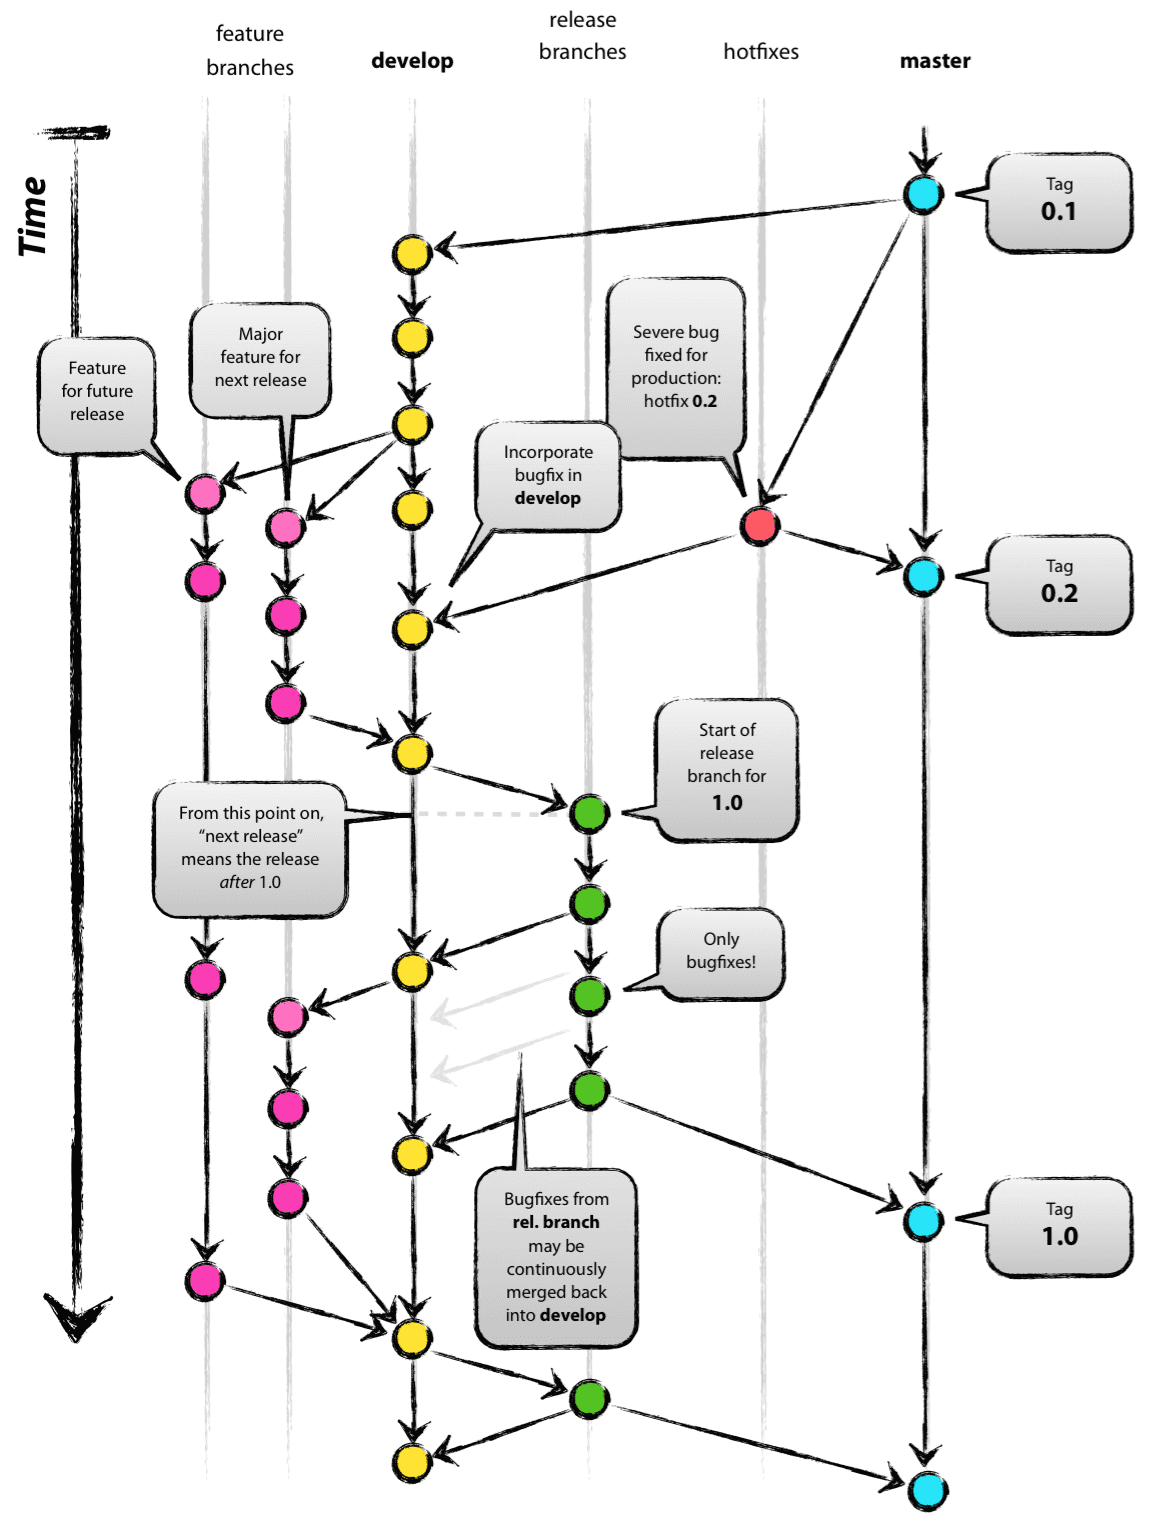
\includegraphics[width=0.85\linewidth]{estrategia}
 	\end{center}
 	\legend{Fonte: (http://nvie.com/posts/a-successful-git-branching-model/)}
 \end{figure}


\section{Os branches}

Na estratégia que iremos adotar vamos trabalhar com seis tipos de ramos, são eles, dois ramos principais e quatro tipos de ramos de apoio. 

Os ramos principais são os ramos \textit{master} e o \textit{develop}. E os ramos de apoio serão os ramos, \textit{feature}, \textit{release}, \textit{hotfix} e \textit{buxfix}. A seguir irei descrever cada um desses ramos. 

%Os ramos principais têm vida infinita, ou seja, eles sempre estarão presentes dentro do desenvolvimento, em contrapartida, os branches de apoio têm vida curta, sendo excluidos após suas utlizações, essas questões ficarão mais claras na prática.

\subsection{O \textit{branch} \textit{master}}

O ramo \textit{master} é o ramo que irá abrigar os códigos em suas versões mais estáveis, esse é o branch de produção. É o ramo que dará origem a aplicação final. Em algum momento do desenvolvimento todos os códigos produzidos em outros ramos farão um \textit{merge}(ato de mesclar os ramos, colocar os arquivos de um \textit{branch} em outro) com o \textit{branch master}, de forma direta ou indireta.

\subsection{O \textit{branch develop}}

Este ramo será responsável por conter os códigos em nível de desenvolvimento para o próximo \textit{deploy}(significa implementar, mas pode mudar de significado de acordo com o contexto). Lembre-se que os códigos não serão criados nesse \textit{branch}, esse é responsável apenas em abrigar os códigos que estão em desenvolvimento. Após os códigos serem devidamente testados, o \textit{branch develop} fará um merge com o \textit{branch master}, isso se nem um \textit{bug} for encontrado no processo de testes, esse processo está representado na figura \ref{develop}. Se o código aprensentar \textit{bug} será criado outro branch a partir do \textit{branch develop} para a correção dos \textit{bugs} e posteriormente mesclado com o \textit{branch master}.

\begin{figure}[h]
	\caption{\label{develop}O \textit{branch} \textit{develop}}
	\begin{center}
		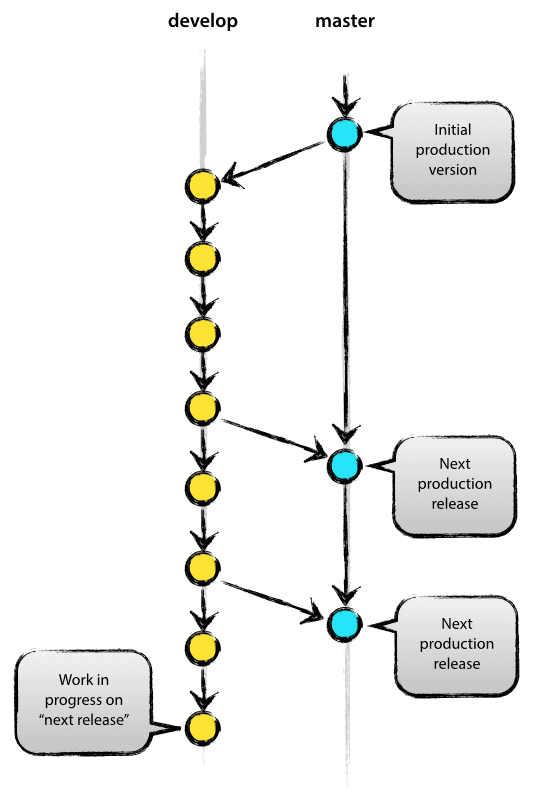
\includegraphics[width=0.6\linewidth]{develop}
	\end{center}
	\legend{Fonte: (http://nvie.com/posts/a-successful-git-branching-model/)}
\end{figure}
	
Os branches \textit{master} e \textit{develop}, possuem vida infinita, ou seja, eles sempre estarão presentes durante o desenvolvimento, e serão criados sempre que o git for inicializado. Os branches a seguir terão vida curta, eles serão criados e após suas utlizações eles serão finalizados e excluídos, esse processo firará mais claro na prática.

\subsection{O \textit{branch} \textit{feature}}

O branch feature representado na figura \ref{feature}, será utlizado sempre que uma nova funcionalidade precisar ser criada. Ele sempre será criado a partir do\textit{ branch develop} e finalizado no \textit{branch develop}, independente em qual ramo você esteja, isso se você estiver utlizando o \textit{git-flow}.

Ao contrário do ramo \textit{master} e \textit{develop}, o ramo \textit{feature} pode ser criado múltiplas vezes, uma para cada nova funcionalidade. Esse branch possui como prefixo \textit{feature/*}, onde o asterisco(*) será substituido pelo nome do "sub-ramo" \ digamos assim, por exemplo, \textit{feature/cadastrodeclientes}, \textit{feature/teladelogin}.

\begin{figure}[h]
	\caption{\label{feature}O \textit{branch} \textit{feature}}
	\begin{center}
		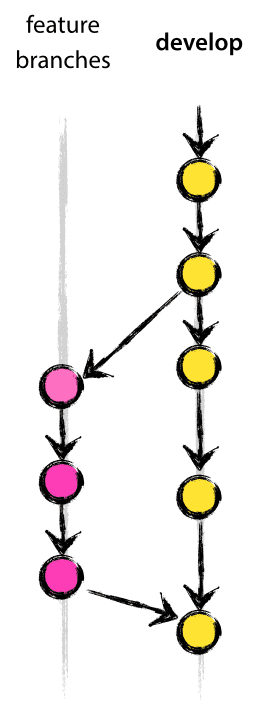
\includegraphics[width=0.26\linewidth]{feature}
	\end{center}
	\legend{Fonte: (http://nvie.com/posts/a-successful-git-branching-model/)}
\end{figure}


São duas as principais maneiras de mesclar branches, figura \ref{feature-merges}. A primeira é fazendo a mesclagem criando um novo \textit{commit} com as alterações dentro do ramo \textit{develop}, sem adicionar os \textit{commits} criados durante o desenvolvimento do ramo feature e, a outra é adicionando os \textit{commits} criados no ramo \textit{feature} dentro do ramo \textit{develop} e, mais um novo \textit{commit} indicando a mesclagem, o git-flow usa como padrão esse último. Novamente, esse proceso ficará mais claro durante a prática.


\begin{figure}[h]
	\caption{\label{feature-merges}Tipos de merges}
	\begin{center}
		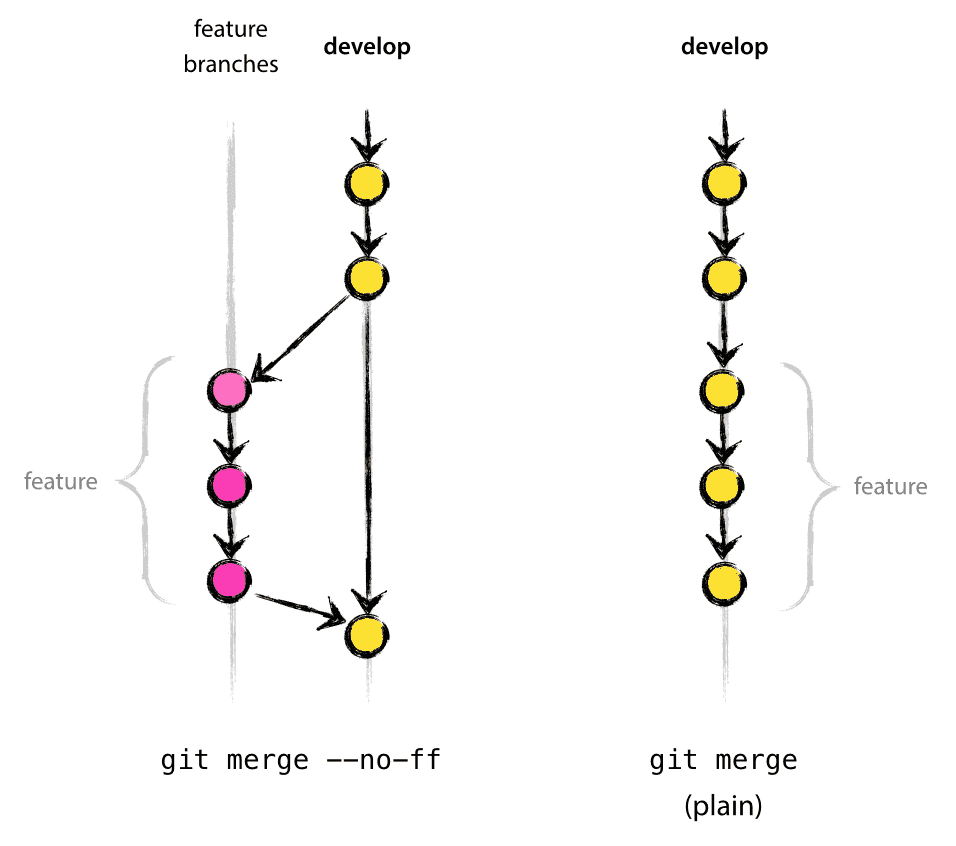
\includegraphics[width=0.8\linewidth]{feature-merges}
	\end{center}
	\legend{Fonte: (http://nvie.com/posts/a-successful-git-branching-model/)}
\end{figure}

\subsection{O \textit{branch release}}

Esse branch é o ramo intermediário entre o \textit{develop} e o \textit{master}. O objetivo desse branch é a criação de tags(são os números que indicam a versão da aplicação, 1.0.0, por exemplo). Ele inicia no \textit{branch develop} e termina no \textit{branch master} e no \textit{develop}. Você deve está se perguntando porquê um \textit{branch} que inicia-se no \textit{develop} tem que terminar no \textit{develop}. Isso acontece porquê o \textit{branch} \textit{develop} tem que ter a mesma \textit{tag} do \textit{branch master}.

O prefixo usado pelo \textit{branch release} é \textit{release/*}\ , onde o asterisco(*) deve ser substituido pela tag da \textit{realese}, por exemplo, \textit{release/0.1.0}. Mais na frente iremos aprender um conjunto de regras para a criação dessas tags, conhecido como versionamento semântico.

Sempre quando falo que um branch "termina"\ ou "finaliza", \ me refiro a mesclagem de um branch em outro, usado por padrão pelo git-flow.

\subsection{Os \textit{branches hotfixes} e \textit{bugfixes}}

O \textit{branch hotfix} e \textit{bugfix}, tem o objetivo de correção de erros. A diferença entre eles é onde cada um é inicializado. 

Se o \textit{bug} for encotrado no ramo de produção(\textit{branch master}), um \textit{branch hotfix}, ver figura \ref{hotfix}, deve ser criado para tratar o erro a partir do ramo \textit{master}. Após a correção do erro, uma nova \textit{tag} será criada automaticamente e, o \textit{branch hotfix} será mesclado com o ramo \textit{master} e também ao ramo \textit{develop} para que esse não apresente o erro em futuras versões.

Análogo ao \textit{branch release}, o prefixo do \textit{branch hotfix} é \textit{hotfix/*}\ , onde o asterisco(*) deve ser substituido pela nova tag, por exemplo, \textit{hotfix/0.1.1}.

\begin{figure}[h]
	\caption{\label{hotfix}O \textit{branch hotfix}}
	\begin{center}
		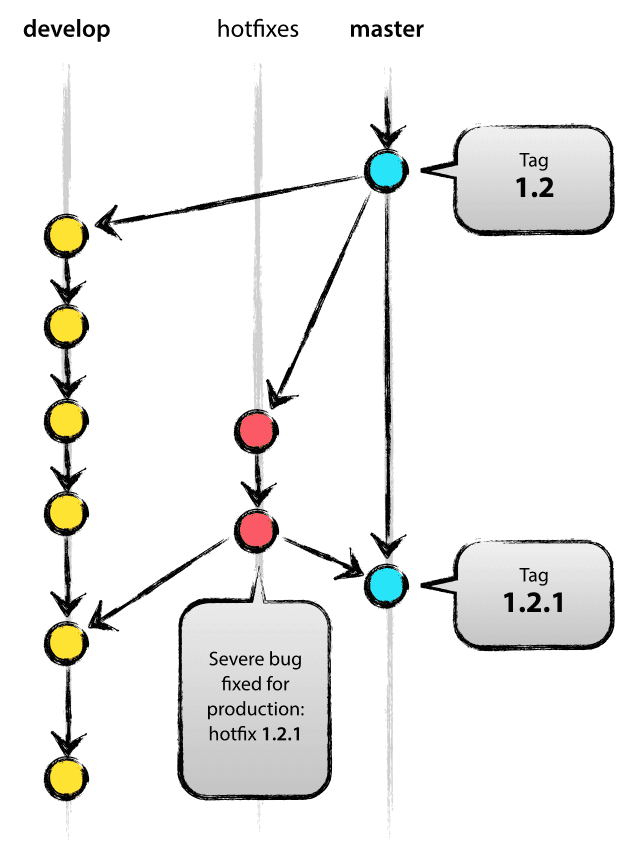
\includegraphics[width=0.6\linewidth]{hotfix}
	\end{center}
	\legend{Fonte: (http://nvie.com/posts/a-successful-git-branching-model/)}
\end{figure}

Já o \textit{branch bugfix}, ele deve ser criado quando um \textit{bug} é encontrado durante o desenvolvimento. Ele é iniciado e finalizado no \textit{branch develop}. Seu prefixo é semelhante ao do \textit{branch feature}, por exemplo, \textit{bugfix/erro-cadastramento}.

\chapter{Primeiros passos com o Git}

Nessa etapa vamos supor que todos estejam com o Git e o Git-flow instalados, caso haja a necessidade de um guia para as instalações, esse será adicionado como apêncide no final livro em futuras versões.

\section{Configuração inicial \label{configinicial}}

O primeiro passo é abrir seu console preferido, se estiverem no Linux ou macOS, abram o terminal. Se estiverem utilizando o Windows, podem utilizar o Git Bash, que é instaldo com o Git. Ainda para usuários Windows, uma dica que eu dou é usar o Cmder, é um console free e muito mais agradável de se trabalhar, e não prescisa ser instaldo, apenas ser baixado, ver figura \ref{cmder}. Sugiro também não utilizar o MS-DOS, nem o PowerShell.

\begin{figure}[h]
	\caption{\label{cmder}Uma alternativa para o MS-DOS, o \textit{Cmder}}
	\begin{center}
		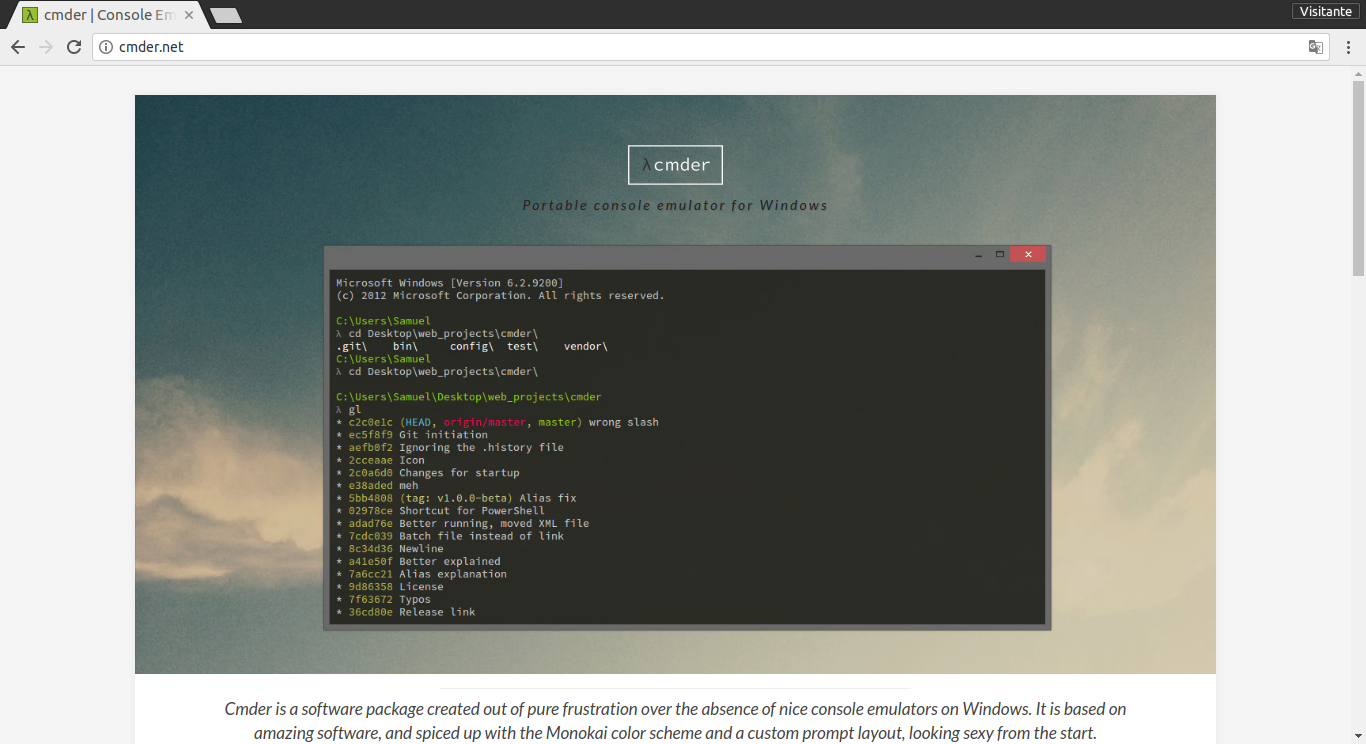
\includegraphics[width=1\linewidth]{cmder}
	\end{center}
	\legend{Fonte: (http://cmder.net/)}
\end{figure}

Com o seu console aberto digite \textit{git}, e aperte enter, isso irá verificar se o git foi instaldo corretamente. Se ele tiver sido instalado corretamente, irá aparecer algo semelhante a figura \ref{terminal}.

\begin{figure}[h]
	\caption{\label{terminal}Verificando a instalação do git}
	\begin{center}
		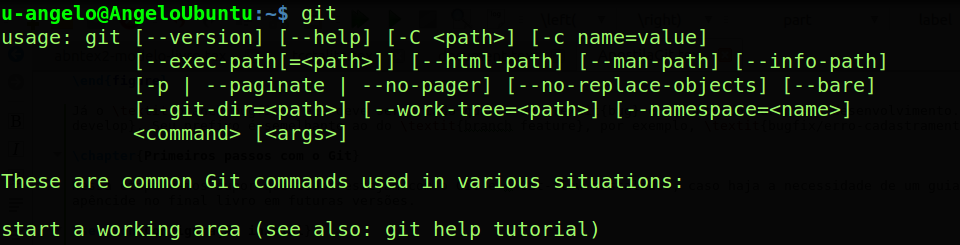
\includegraphics[width=1\linewidth]{terminal}
	\end{center}
	\legend{Fonte: (Do autor)}
\end{figure}

Com o git devidamente instalado, vamos começar a configuração. Para isso insira os seguintes comandos, o primeiro será para o git identificar seu nome, e o segundo seu email(figura \ref{configuracao}):

	\begin{verbatim}
		          git config --global user.name "Angelo Medeiros"
		          git config --global user.email "angelo@email.com"
	\end{verbatim}

Caso queira visualizar suas configuração globais, digite o comando:

\begin{verbatim}
		          git config --global --list
\end{verbatim}

O próximo comando serve para facilitar o entendimento visual:

		\begin{verbatim}
		          git config --global color.ui true
		\end{verbatim}

\begin{figure}[h]
	\caption{\label{configuracao}Configuração inicial do git}
	\begin{center}
		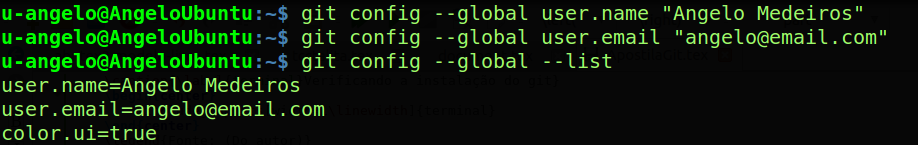
\includegraphics[width=1\linewidth]{configuracao}
	\end{center}
	\legend{Fonte: (Do autor)}
\end{figure}

\chapter{Os 3 estágios}

Nesse capítulo ensinarei a criar seu primeiro repositório git. E quais são os três principais estágios do processo para o versionamento usado pelo git.

\section{Criando um repositório}

O primeiro passo é acessar a pasta que você quer iniciar o repositório git. Para exemplificar eu criei uma pasta chamada gitLegal, e usei os seguintes comandos(ver figura \ref{repositorio}):

\begin{verbatim}
		        Criando a pasta gitLegal: mkdir gitLegal
		        Acessando a pasta criada: cd gitLegal
		        Verificando o conteudo da pasta: ls
		        Iniciando o repositório git: git init
		        Verificando novamente a pasta: ls
		        Verificando a existência de arquivos ocultos: ls -a
\end{verbatim}

\begin{figure}[h]
	\caption{\label{repositorio}Criando repositório git}
	\begin{center}
		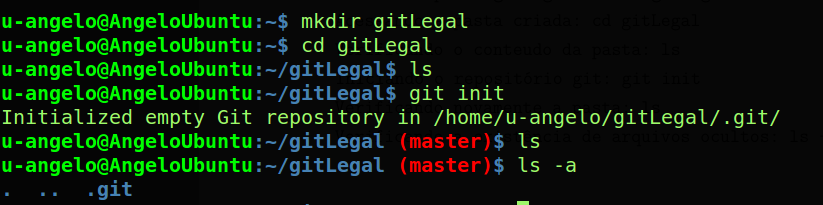
\includegraphics[width=1\linewidth]{repositorio}
	\end{center}
	\legend{Fonte: (Do autor)}
\end{figure}

O processo de verificação da pasta foi feito apenas para mostrar que quando o repositório é inicializado o git cria uma pasta oculta. Nessa pasta oculta estão todos os arquivos necessário para o git gerenciar seu repositório. Na prática você usará apenas o comando \textit{git init}.

\section{O primeiro estágio}

O primeiro estágio é chamado de "untracked files". Assim que você faz alguma aleteração no repositório, cria uma pasta ou arquivo, ou altera um arquivo, isso faz com que o elemento que você alterou entre no primeiro estágio.

Para verificar em que estágio seus elementos estão, basta digitar o comando \textit{git status}.

Se for dado um \textit{git status} na pasta gitLegal, não irá aparecer nada, pois o repositório não teve nemnhuma alteração. 

Para demonstrar o primeiro estágio irei criar um arquivo em branco chamado \textit{helloWorld} e, em seguida, executarei o comando para verificar o estágio(ver figura \ref{estagio1}).

\begin{figure}[h]
	\caption{\label{estagio1}O primeiro estágio}
	\begin{center}
		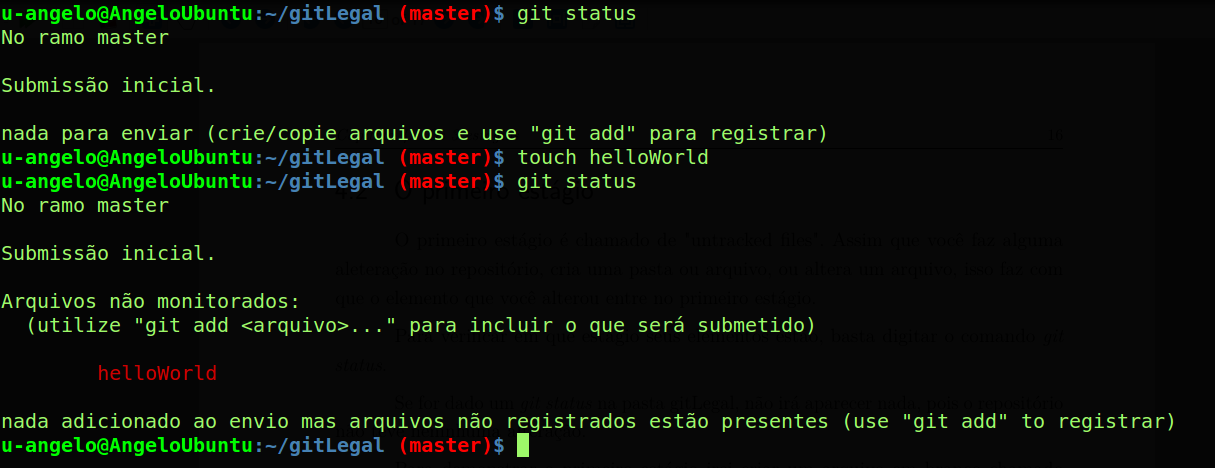
\includegraphics[width=1\linewidth]{estagio1}
	\end{center}
	\legend{Fonte: (Do autor)}
\end{figure}

O comando \textit{touch} foi usado para a criação do arquivo \textit{helloWorld}.

\section{O segundo estágio}

O segundo estágio é chamado de "Changes to be committed". Nessa etapa você irá adicionar os elementos do primeiro estágio para serem "commitados" \ no terceiro estágio. Irei criar outro arquivo em branco, chamado helloWorld2, apenas para ficar mais claro a importância dessa etapa(ver figura \ref{estagio2}).

\begin{figure}[h]
	\caption{\label{estagio2}O segundo estágio}
	\begin{center}
		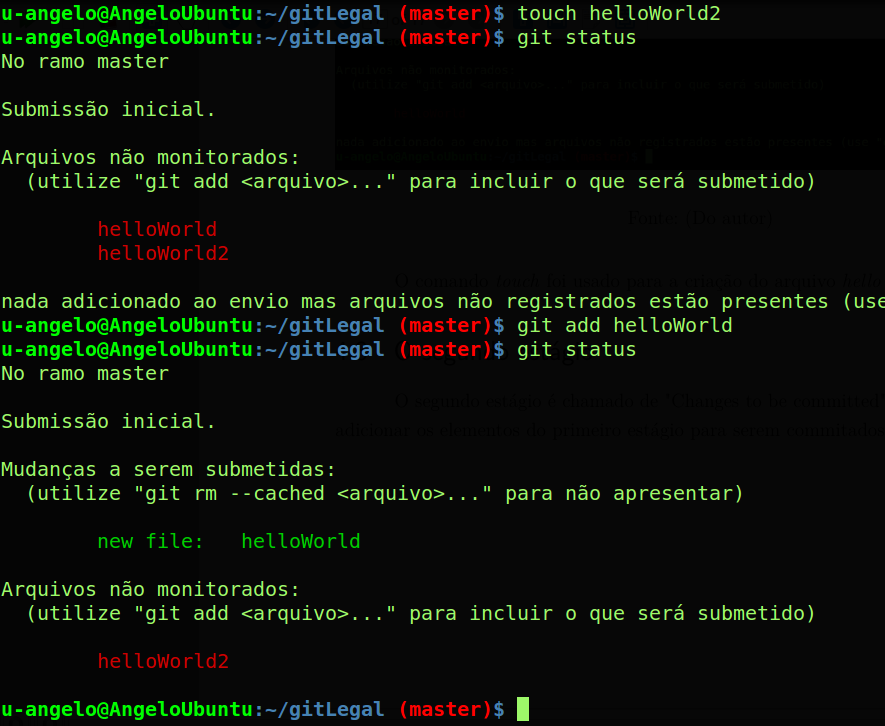
\includegraphics[width=1\linewidth]{estagio2}
	\end{center}
	\legend{Fonte: (Do autor)}
\end{figure}

Agora vamos entender o que foi feito. Com a adição do arquivo helloWorld2, o primeiro estágio agora tem dois elementos. Vamos supor que você queira adicionar apenas o primeiro helloWorld world para o último estágio. Para fazer isso, foi necessário apenas usar o comando \textit{git add helloWorld}.

Como mostra a figura \ref{estagio2}, no segundo estágio encontra-se apenas o primeiro \textit{helloWorld}. Peço desculpas pela falta de criatividade ao nomear os elementos.

Na maioria das vezes é necessário adicionar mais de uma arquivo ao terceiro estágio e não é viável adicionar um por um. Uma alternativa mais eficiente para essa situação é usar o comando "\textbf{git add .}", ele irá adicionar todos os arquivos ao terceiro estágio. Preste atenção no ponto seguido do add, ele também faz parte do comando.

\section{O terceiro estágio}

Nesse estágio é onde acontece o famoso \textit{commit}. Para quem não sabe o que é um \textit{commit}, ele nada mais é que um \textit{snapshot} do estado de sua aplicação. Na figura \ref{estagio3} mostra o arquivo \textit{helloWorld} sendo "commitado". Observe que após o \textit{commit}, o arquivo \textit{helloWorld} não aparece mais quando é usado o comando \textit{git status}. O arquivo só voltará a aparecer quando sofrer alguma alteração novamente. 

\begin{figure}[h]
	\caption{\label{estagio3}O terceiro estágio}
	\begin{center}
		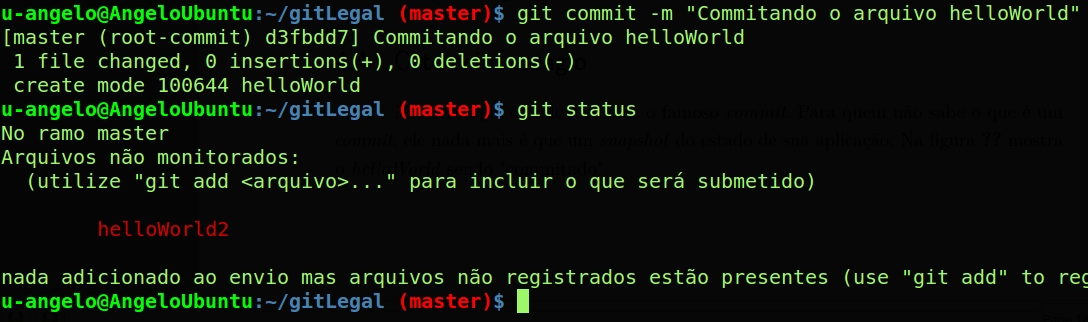
\includegraphics[width=1\linewidth]{estagio3}
	\end{center}
	\legend{Fonte: (Do autor)}
\end{figure}

Existem duas principais maneiras de realizar um \textit{commit}, na figura \ref{estagio3} mostra uma delas. Na figura \ref{commit} mostrarei a outra maneira realizando um \textit{commit} do \textit{helloWorld2}. 

\begin{figure}[h]
	\caption{\label{commit}Outra maneira de realizar um commit}
	\begin{center}
		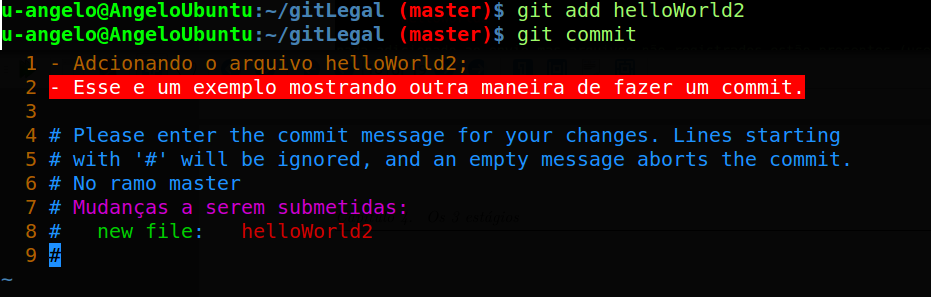
\includegraphics[width=1\linewidth]{commit2}
	\end{center}
	\legend{Fonte: (Do autor)}
\end{figure}

A primeira maneira deve ser usada quando você fez poucas alterações, e você consegue descrever todas esses mudanças em apenas uma linha usado o commando \textit{git commit -m "comentario"}. A segunda maneira deve ser usada quando for preciso descrever diversas alterações e apenas uma linha não basta. Uma dica é, evite usar acentuação dentro dos comentários, quando a acentuação é usada, algumas vezes quando você for visualizar os commits, a acentuação poderá não ser reconhecida pelo console.

\chapter{Comandos mais usados no git}

Nesse capítulo irei apresentar os principais comandos usados pelo git, e sempre estarei dando algumas dicas.

\section{Visualizando o log}

Até agora vocês aprenderam a visualizar em que estágio está sua aplicação, e a criar os \textit{commits}. Agora ensinarei como visualizar os \textit{commits} criados, o \textit{log}. O comando básico para visualizar um \textit{log} é o \textit{git log}(ver figura \ref{gitlog}), mas ele também pode vim com outras opções, ensinarei os mais usados.

\begin{figure}[h]
	\caption{\label{gitlog}Visualizando o log básico}
	\begin{center}
		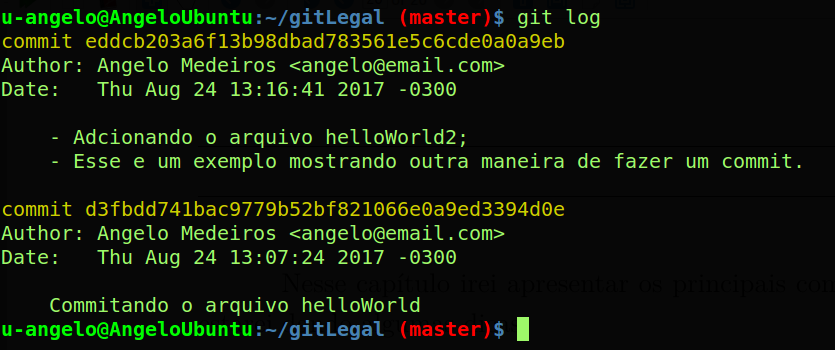
\includegraphics[width=1\linewidth]{gitlog}
	\end{center}
	\legend{Fonte: (Do autor)}
\end{figure}

Irei adicionar dentro do arquivo helloWorld, o texto a seguir e fazer um novo commit. 

\begin{verbatim}
          # Comando para imprimir na tela usando o python 2.x 
                   
          print "Hello world!"
\end{verbatim}

A figura \ref{pretty} mostra a execução do commando \textit{git log --pretty=oneline}. Esse comando exibe o log de forma reduzida, mostrando apenas o \textit{hash} e os comentários em apenas uma linha.

\begin{figure}[h]
	\caption{\label{pretty}Outra maneira de visualizar o log}
	\begin{center}
		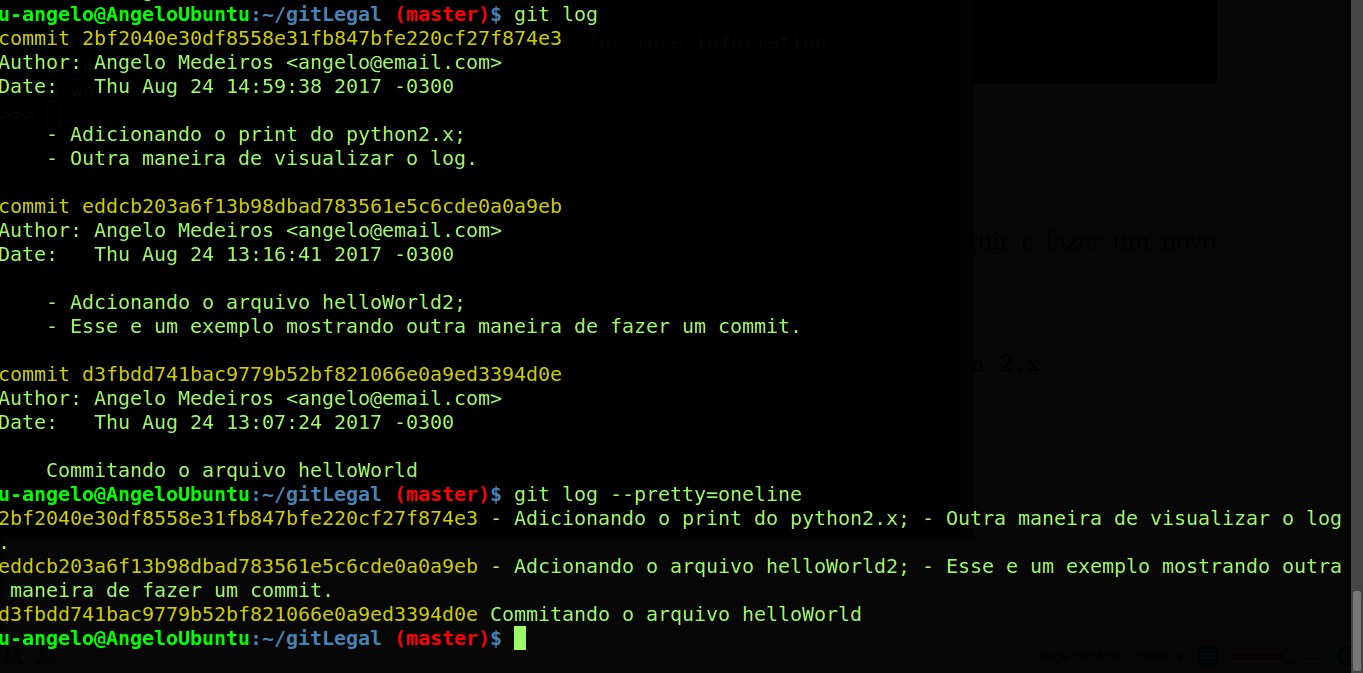
\includegraphics[width=1\linewidth]{pretty}
	\end{center}
	\legend{Fonte: (Do autor)}
\end{figure}

Outra opção para o mesmo comando é:

\begin{itemize}
	\item \verb|git log --pretty=oneline -2|, o parâmetro -2, faz com que o comando exiba apenas os dois últimos commits(você pode alterar o parâmetro por qualquer outro valor).
\end{itemize}

Abaixo seguem outros comandos para vocês experimentarem:

\begin{itemize}
	\item \verb|git log -p|, exibe as alterãções em cada arquivo de todos os commits;
	\item \verb|git log -p -1|, exibe as alterãções do último commit(ver figura \ref{logp});
	\item \verb|git log --stat|, exibe um resumo das alterações;
	\item \verb|git log --stat -2|, exibe um resumo das alterações dos últimos dois commits;
	\item \verb|git log --since=10.minutes|, exibe os commits dos últimos 10 minutos;
	\item \verb|git log --since=2.hours|, exibe os commits das últimas duas horas;
	\item \verb|git log --since=1.days|, exibe os commits no intervalo de tempo de um dia.
\end{itemize}


\begin{figure}[H]
	\caption{\label{logp}Mais uma maneira de visualizar o log}
	\begin{center}
		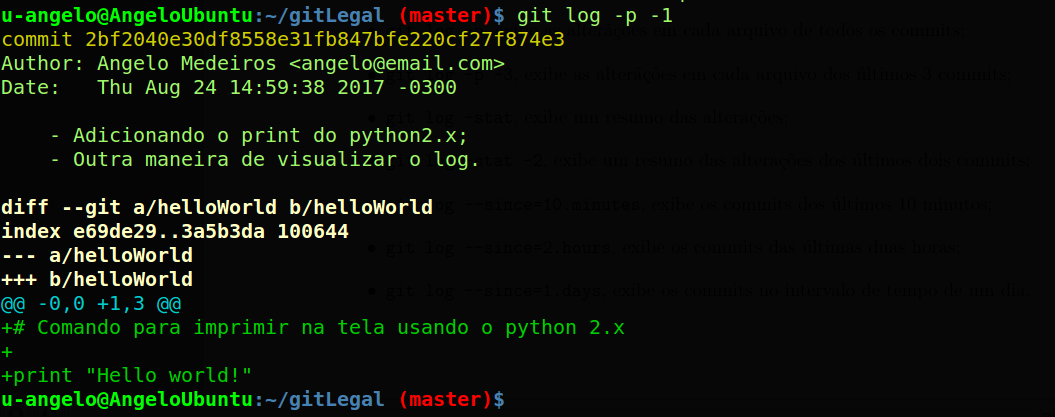
\includegraphics[width=1\linewidth]{logp}
	\end{center}
	\legend{Fonte: (Do autor)}
\end{figure}

Na figura \ref{logp} as linhas que começam com um símbolo de mais(+) indica alg:wo que foi adicionado. Se começar com o símbolo de menos($-$) significa que algo foi retirado. Os números entre os símbolos de (@), indicam as posições das linhas, onde houveram alterações. Quando vocês estiverem praticando, isso ficará mais claro.

\section{Criando branches \label{criandobranch}}

Para criar um novo \textit{branch}, usamos o comando \textit{git checkout -b nomeBranch}. Onde \textit{nomeBranch} deve ser substituído pelo nome do \textit{branch} que você quer criar. Vale resaltar que um \textit{branch} é sempre criado baseado no \textit{branch} atual, ou seja, se você estiver no\textit{ branch master}, o novo \textit{branch} será um clone do \textit{branch master}, ver figura \ref{novobranch}.

\begin{figure}[H]
	\caption{\label{novobranch}Criando um branch}
	\begin{center}
		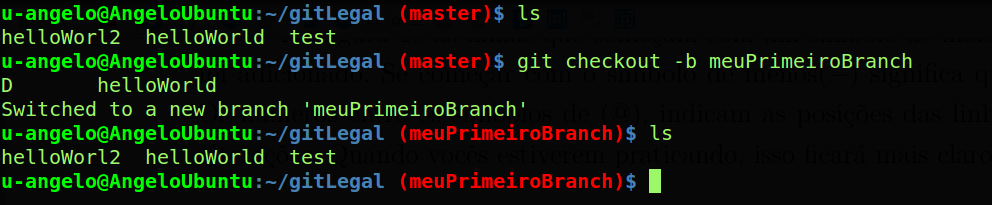
\includegraphics[width=1\linewidth]{novobranch}
	\end{center}
	\legend{Fonte: (Do autor)}
\end{figure}

Observe que quando você cria um \textit{branch}, o \textit{git} já inicia dentro do novo \textit{branch}. Irei listar abaixo os principais comandos relacionados a manipulação dos branches.

\begin{itemize}
	\item \verb|git checkout nomeDoBranch|, troca do \textit{branch} atual para o \textit{branch nomeDoBranch};
	\item \verb|git branch|, exibe os branches criados localmente;
	\item \verb|git branch -a|, exibe os branches locais e os remotos(se você tiver trabalhano com branches remotos);
	\item \verb|git branch -d nomeDoBranch|, deleta o \textit{branch nomeDoBranch}.
\end{itemize}

\section{Mesclando branches}

Mesclar branches na maioria das vezes é uma tarefa fácil. Porém algumas vezes ocorrem conflitos, esse assunto será tratado em uma seção mais na frente. Por enquanto, vamos se preocupar apenas em mesclar os \textit{branches}. São duas as principais maneiras de fazer a mesclagem usando o git, você pode usar o \textit{merge} ou o \textit{rebase}.

\subsection{Mesclando usando o merge}

O comando $$\verb|git merge funcionalidade1|$$ é usado para realizar o merge. Ele irá mesclar o \textit{branch funcionalidade1} com o \textit{branch atual}.

A vantagem do merge é que ele preserva um histórico completo do seu projeto e, evita problemas quando está trabalhando em equipe(ver figura \ref{merge}).

\begin{figure}[H]
	\caption{\label{merge}Mesclando usando o merge}
	\begin{center}
		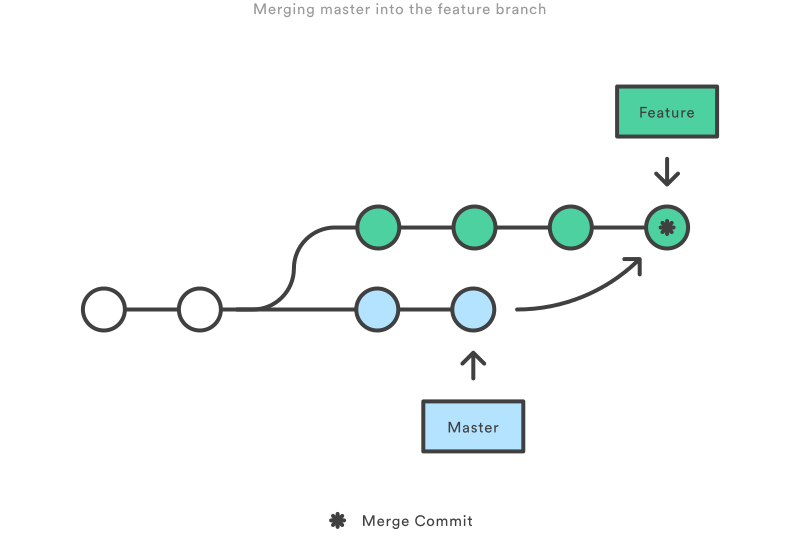
\includegraphics[width=0.5\linewidth]{merge}
	\end{center}
	\legend{Fonte: (https://stackoverflow.com/questions/16666089)}
\end{figure}

\subsection{Mesclando usando o rebase}

O rebase preserva um histórico mais limpo e linear do seu projeto, porém ao trabalhar em grupo isso torna-se uma desvantagem, pois o rebase recria os commits. Na figura \ref{rebase} quando o elemento E foi mesclado com o elemento D dando origem ao elemento R, o elemento E foi reescrito com outro commit, isto é, com outro hash. Então para alguém de fora que tenha o elemento E vai ter um commit diferente do seu, apesar de ser o mesmo elemento, tornando algo confuso.

\begin{figure}[H]
	\caption{\label{rebase}Mesclando usando o rebase}
	\begin{center}
		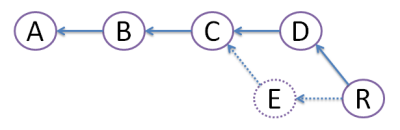
\includegraphics[width=0.5\linewidth]{rebase}
	\end{center}
	\legend{Fonte: (https://stackoverflow.com/questions/16666089)}
\end{figure}

O rebase é aconselhado apenas quando você está trabalhando localmente, a não ser que você saiba o que está fazendo. Caso contrário, use sempre o merge. A documentação do git descreve diversos parâmetros que podem e devem ser usados, tanto para o rebase e para o merge.

\section{Voltando versões}

Na minha opinião essa é a principal função do git, o processo de voltar versões. Existem diversas maneiras de fazer isso. Algumas são simples, mas não oferecem muita segurança para quem está iniciando nesse novo mundo do controle de versões. Outras envolvem mais etapas, porém você sentirá segurança realizando o processo,  o fato de ter mais etapas não o torna mais difícil.

A maioria dos comandos para voltar versões necessitam do \textit{hash} do \textit{commit}, você pode encontrar esse \textit{hash} visualizando o \textit{log}. Não é necessário o hash completo, apenas o começo. A seguir estão os principais comandos:

\begin{itemize}
	\item \verb|git reset d3fbdd741 --hard|, desfaz todas as alterações anteriores do commit d3fbdd741(ver figura \ref{voltando});
	\item \verb|git reset HEAD~2 --hard|, desfaz todas as alterações dos dois últimos commits;
	\item \verb|git ckeckout d3fbdd741|, cria um branch temporário a partir do commit d3fbdd741.
\end{itemize}

\begin{figure}[h]
	\caption{\label{voltando}Voltando versão}
	\begin{center}
		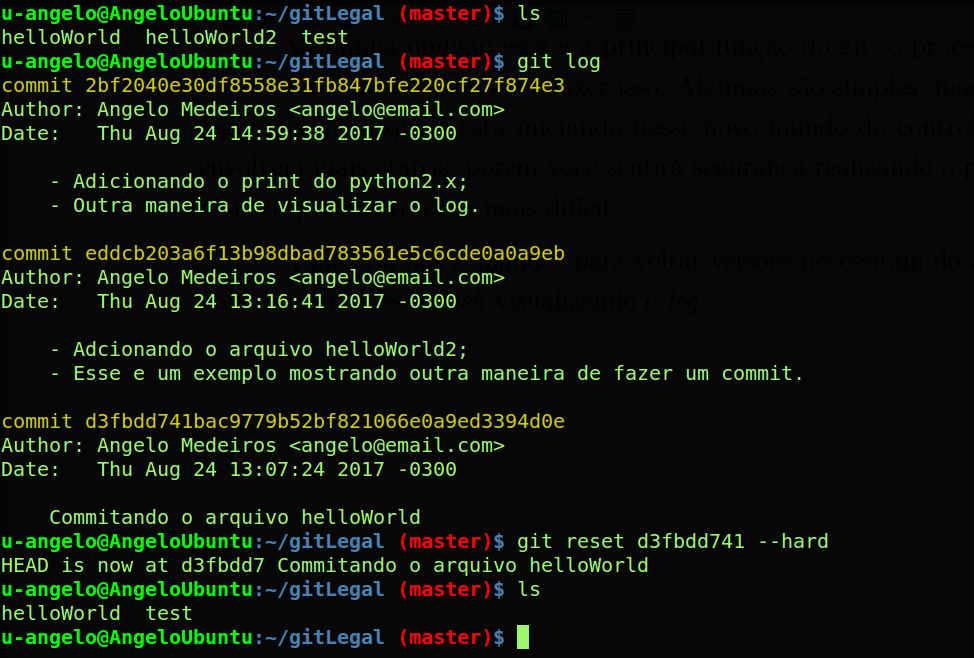
\includegraphics[width=1\linewidth]{voltando}
	\end{center}
	\legend{Fonte: (Do autor)}
\end{figure}

Entendo a figura \ref{voltando}. Veja que antes do \textit{reset} existia o arquivo \textit{helloWorld2}. No final do processo além de apagar o arquivo \textit{helloWorld2}, as alterações feitas no arquivo \textit{helloWorld} também foram desfeitas, apesar de não mostrar na figura. Essas mudanças aconteceram porquê o arquivo \textit{heloWorld2} foi criado no \textit{commit} eddcb203a, como pode ser observado nos comentários do \textit{commit} mostrado no \textit{log}, e o conteudo do arquivo \textit{helloWorld} ocorreu no \textit{commit} 2bf2040e30. Por isso a importância de documentar corretamenta os \textit{commits}.

Você pode combinar diversas técnicas para voltar versões usando o git. Quando forem ganhando mais segurança do que estão fazendo, o processo de voltar versões irá se tornar algo natural. Por exemplo, você pode criar um novo \textit{branch} a partir do qual queira voltar uma versão, e depois mesclar esse novo \textit{branch} com o \textit{branch} principal. Depende apenas da sua engenhosidade, então façam diversos experimentos usando o git para adquirir experiência.

\section{Algumas dicas}

Nas seções seguintes serão descritas algumas dicas.

\subsection{Ignorando arquivos com o Git}

Geralmente tem arquivos que são criados automaticamente durante um projeto, por exemplo arquivos de log. Tais arquivos sempre ficam aparecendo no segundo estágio e isso não é algo interessante. 

Para impedir que alguns arquivos fiquem aparecendo ao visualizar o status, o git trabalha com o arquivo \textbf{.gitignore}. Esse arquivo é criado na raiz do projeto e, contém os nomes dos arquivos a serem ignorados, ver figura \ref{gitignore}. 

\begin{figure}[h]
	\caption{\label{gitignore}Ignorando arquivos}
	\begin{center}
		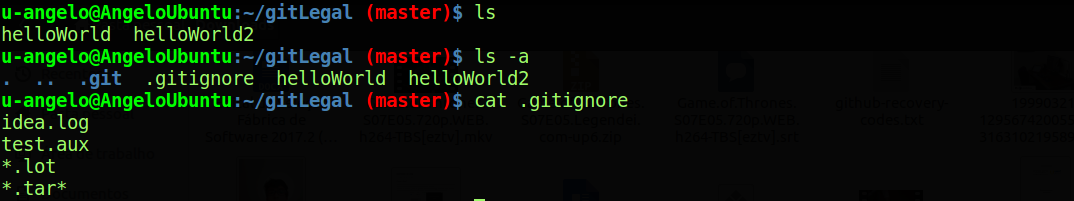
\includegraphics[width=1\linewidth]{gitignore}
	\end{center}
	\legend{Fonte: (Do autor)}
\end{figure}

No exemplo da figura \ref{gitignore}, os arquivos \textit{idea.log} e \textit{test.aux}, não aparecerão mais no status. Todos os arquivos que terminarem com a extensão \textbf{.lot} ou apresentarem a extensão \textbf{.tar}, por exemplo \textit{ubuntuMobile.tar.xz}, também serão ignorados. 

\textit{\textbf{Observação:}} Se um arquivo já tiver sido adicionado para o segundo estágio em algum momento do desenvolvimento, ele não será ignorado, mesmo que o nome do arquivo esteja presente no \textbf{.gitignore}. Se esse for o caso, o comando $$\verb|git rm --cached nomeDoArquivo|$$ irá retirar o arquivo do segundo estágio, ou seja, do monitoramento e, a partir disso ele passará a ser ignorado normalmente, caso queira retirar uma pasta completa, use o comando $$\verb|git rm -r --cached nomeDaPasta|$$ experimente ambos como prática.


\subsection{Alterando o proxy \label{alterandoproxy}}

Dependendo do local onde esteja trabalhando, é necessário uma configuração prévia do proxy para o git trabalhar com repositórios remotos. 

Os principais comandos para alteração do proxy são:

\begin{itemize}
	\item \verb|git config --global http.proxy "proxy:port"|
	\item \verb|git config --global http.proxy "10.10.32.1:3128"|, altera o proxy para  10.10.32.1 na porta 3128
	\item \verb|git config --global http.proxy ""|, altera o proxy de \textit{manual} para \textit{nenhum}
	\item  \verb|git config --global --unset http.proxy|, outra maneira para desativar o proxy
\end{itemize}


\chapter{Trabalhando com repositório remoto}

Na seção \ref{gitlab} falei brevemente sobre o \textit{gitLab}, Nesse capítulo iremos estudar como o \textit{git} se comporta trabalhando com repositórios remotos e faleremos sobre algumas características do \textit{gitLab}.

Antes de começar a usar os comandos das próximas seções, será necessário a criação de uma conta no \textit{gitLab}.

\section{Criando seu primeiro repositório remoto}

Com o \textit{gitLab} aberto siga as intruções da figura \ref{criandorep1} para iniciar o processo de criação do seu primeiro repositório. Em \textbf{\textit{1}} você irá abrir as opções para a criação do novo repositório. Em \textbf{\textit{2}} você irá selecionar \textit{New project}, a continuação segue nas figuras subsequentes.

\begin{figure}[h]
	\caption{\label{criandorep1}Criando repositório - 1ª etapa}
	\begin{center}
		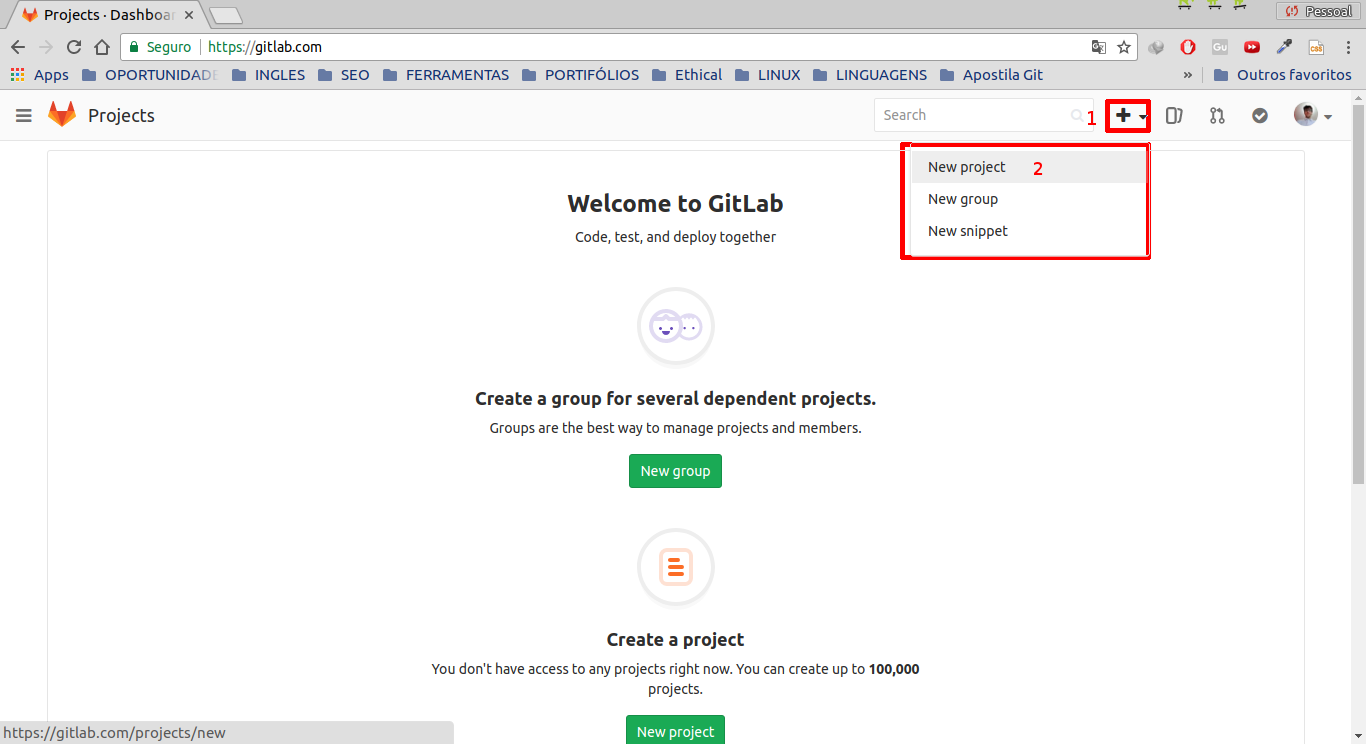
\includegraphics[width=1\linewidth]{criandorep1}
	\end{center}
	\legend{Fonte: (Do autor)}
\end{figure}

Continuando na figura \ref{criandorep2}, em \textbf{\textit{1}} você irá adicionar o nome do repositório, não necessariamente sendo igual ao repositório local. Em \textbf{\textit{2}} exibe as opções de visibilidade do projeto, não tendo relação alguma com as permissões do projeto. Em \textbf{\textit{3}} aperte em \textit{Create project}.

\begin{figure}[h]
	\caption{\label{criandorep2}Criando repositório - 2ª etapa}
	\begin{center}
		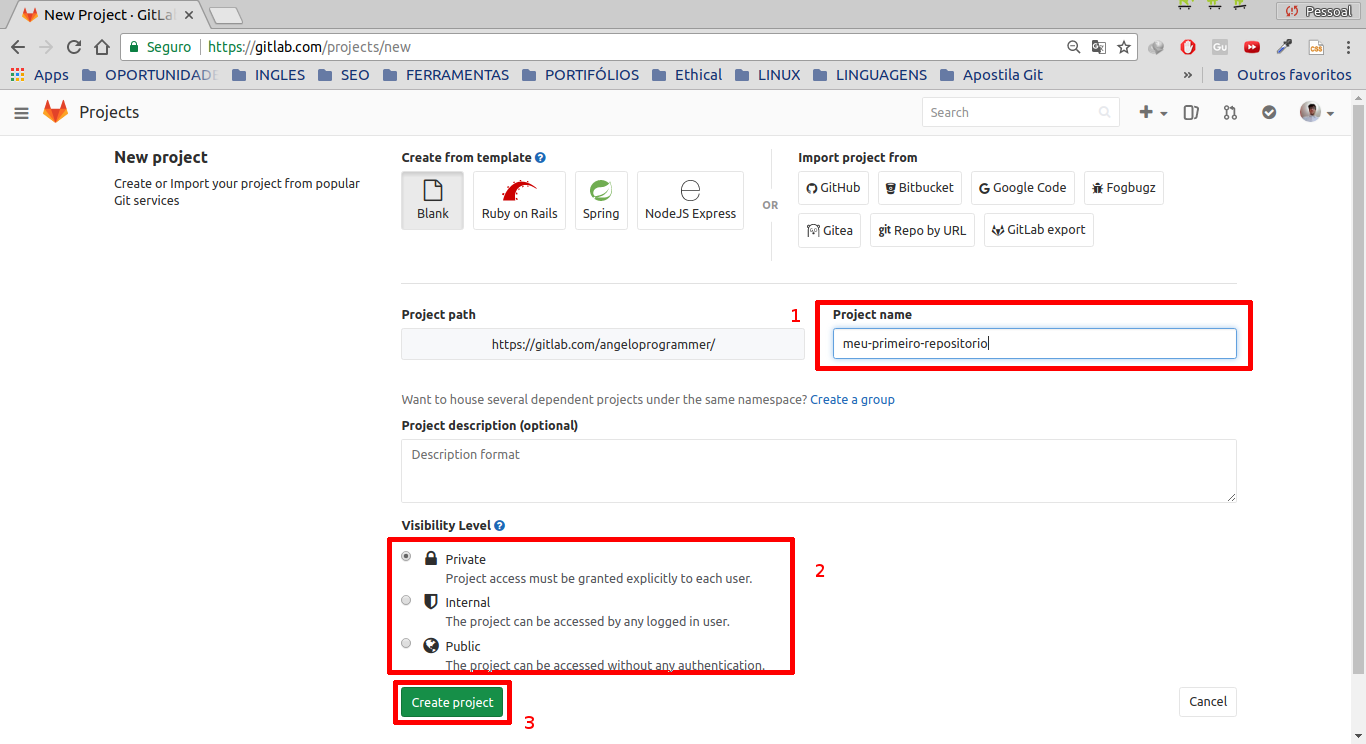
\includegraphics[width=1\linewidth]{criandorep2}
	\end{center}
	\legend{Fonte: (Do autor)}
\end{figure}

O \textit{git} pode se comunicar com os repositórios remotos atráves de dois tipos de protocolos, podendo ser o \textit{HTTPS} e o \textit{SSH}. Com o \textit{HTTPS} não é necessário uma configuração prévia (salvas algumas exceções, como o proxy, dependendo do caso) para iniciar seu uso, enquanto o \textit{SSH} só irá funcionar se você adicionar sua chava pública \textit{SSH} nas configurações do \textit{gitLab}.

Em \textbf{\textit{1}} na figura \ref{criandorep3}, você pode escolher o tipo de protocolo que você irá usar para conectar seu repositório local com o remoto. Em \textbf{\textit{2}}  você pode manipular seu repositório remotamente, criando novos arquivos, novos branches, informando problemas, entre outras opções. Lembre-se que as alterações feitas no repositório remoto não altera o conteúdo do repositório local, a não ser que você utlize comandos no \textit{git} para isso, um \textit{git pull} por exemplo (esse comando será descrito mais a frente).

\begin{figure}[h]
	\caption{\label{criandorep3}Criando repositório - 3ª etapa}
	\begin{center}
		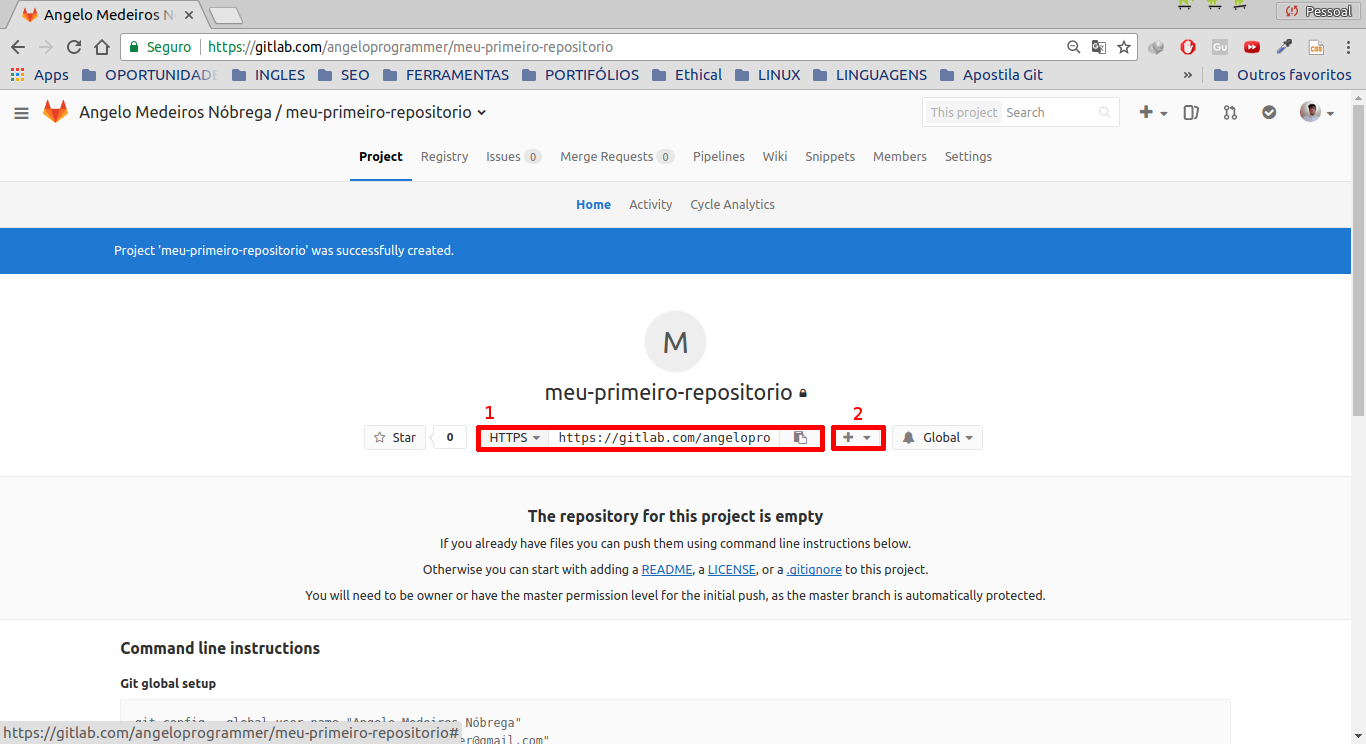
\includegraphics[width=1\linewidth]{criandorep3}
	\end{center}
	\legend{Fonte: (Do autor)}
\end{figure}

Se você observar o \textit{git} está sempre dando dicas. Com o \textit{gitLab} não é diferente. Um exemplo disso está representado na figura \ref{criandorep4}. O \textit{gitLab} exibe diversas opções para você conectar seu repositório remoto com o repositório local. 

Na primeira etapa da figura \ref{criandorep4} você irá realizar a configuração inicial do git, se você vem seguindo a apostila desde os primeiros capítulos, esse processo de configuração já foi realizado na seção \ref{configinicial}. As etapas 2, 3 e 4, serão casos situacionais. 

A etapa 2 deve ser usada quando não existe um repositório local. A primeira linha da etapa 2 irá criar um repositório local, a partir do repositório remoto, na pasta atual em que seu console se encontra. A segunda linha serve para acessar a pasta do repositório. A terceira linha (opcional) criará um arquivo em branco com o nome \textit{README.md}. A quarta linha como já devem saber adiciona o arquivo \textit{README.md} para o terceiro estágio. A quinta linha realizará o commit. E a última linha irá adionar o arquivo \textit{README.md} que foi criado localmente para o repositório remoto, ao \textit{branch master} remoto.

A etapa 3 deve ser utilizada quando você quer iniciar um repositório local e, em seguida fazer a conexão do repositório criado localmente com o repositório remoto. A primeira linha serve para acessar a pasta do repositório. A segunda é utlizada para criar o repositório local. A terceira linha será responsável em estabelecer a conexão entre o repositório local e o remoto. As linhas seguintes vocês já sabem suas devidas aplicações.

A etapa 4 deve ser usada quando já existe um repositório criado localmente. Novamente, a segunda linha irá estabelecer a conexão entre os repositórios. A terceira linha adionará todos os branches locais ao repositório remoto. A quarta linha (opcional) irá adiconar todas as tags criadas, caso existam.

Lembre-se de verificar os tipos de protocolos que estão utilizando. Se tiver em dúvida em qual utilizar opte pelo protocolo \textit{HTTPS}. Lembre-se também de configurar o proxy do seu local de trabalho caso seja necessário.

\begin{figure}[h]
	\caption{\label{criandorep4}Criando repositório - 4ª etapa}
	\begin{center}
		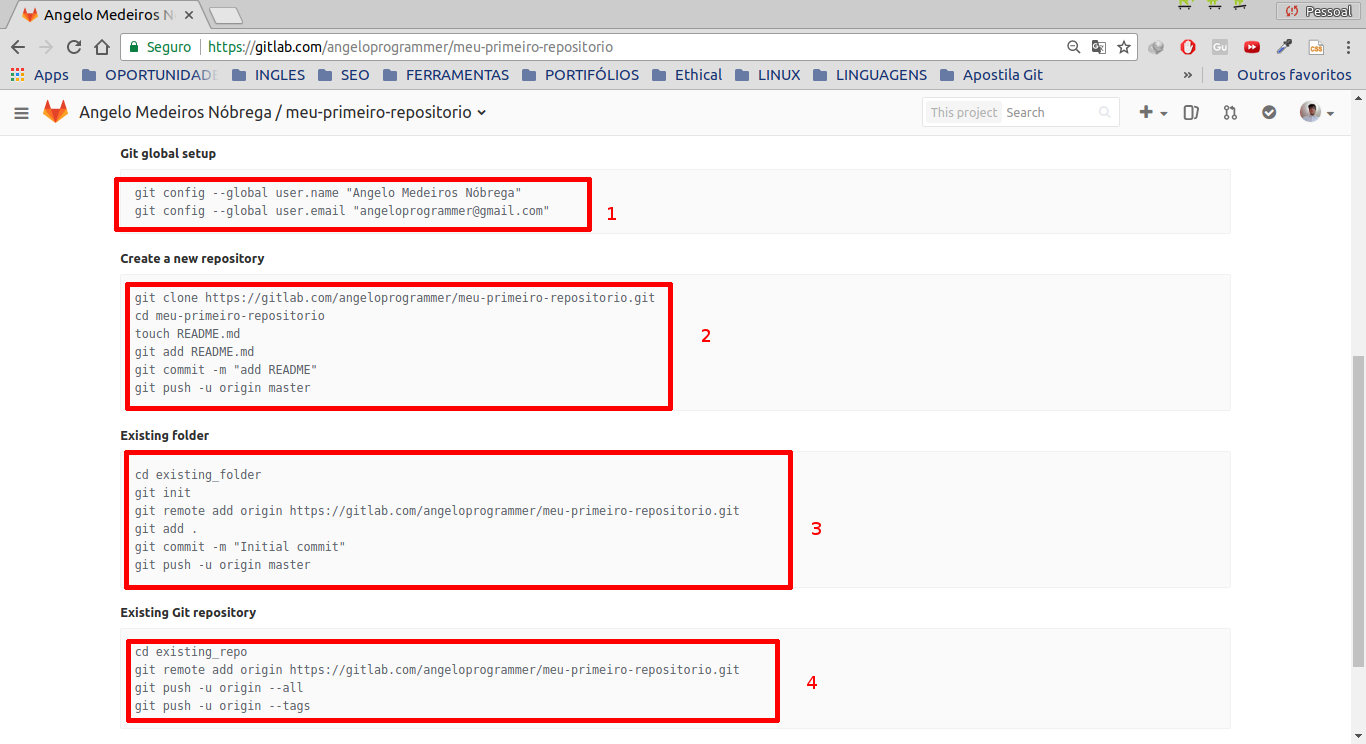
\includegraphics[width=1\linewidth]{criandorep4}
	\end{center}
	\legend{Fonte: (Do autor)}
\end{figure}

\section{Realizando seu primeiro \textit{push}}

O push (empurrar) é o ato de fazer o upload do seu projeto local para um repositório remoto. O \textit{push} só funcionará corretamente se o seu repositório local estiver conectado com o repositório remoto. Essa conexão é realizada com um comando do tipo \verb|git remote add origin ENDEREÇO_DO_REPOSITÓRIO_REMOTO|, esse endereço encontra-se na primeira etapa da figura \ref{criandorep3}. O \textit{origin} não faz parte do comando, ele é o nome padrão dados aos repositórios remotos, mas nada impede de você utlizar outro nome, o aconselhado pela comunidade é manter como \textit{origin}.

Os principais comandos para realizar um push serão descritos a seguir:

\begin{itemize}
	\item \verb|git push -u origin master|, sobe o \textit{branch master} para o repositório remoto, usei como exemplo o master, mas você pode usar qualquer outro \textit{branch} que tenha criado;
	\item \verb|git push -u origin cadastroDeUsuarios|, sobe o branch cadastro de usuários;
	\item \verb|git push -u origin --tags|, sobe as tags criadas (haverá uma seção apenas para tags).
\end{itemize}

\section{Realizando seu primeiro clone}

Realizar um clone é necessário quando você precisa duplicar um repositório remoto para sua máquina. Por exemplo, quando você deleta seu repositório local, ou quando você encontra um projeto opensource e quer utilizá-lo, ou ainda mesmo quando alguém rouba sua máquina e seu projeto está nele, mas nesse último caso só irá funcionar se você estiver usando o git corretamente.

Para fazer um clone é necessário apenas duas condições, o endereço do repositório e obviamente permissão para fazer tal processo. Se o projeto for público você pode fazer o clone do repositório sem pedir a permissão ao dono. Abaixo segue os dois principais comandos para realizar um clone:

\begin{itemize}
	\item \verb|git clone ENDEREÇO_DO_REPOSITÓRIO_REMOTO|
	\item \verb|git clone https://gitlab.com/.../meu-primeiro-repositorio.git|, irá fazer um clone e copiar seus arquivos para a pasta com o nome do repositório, nesse caso \textit{meu-primeiro-repositorio.git};
	\item \verb|git clone https://gitlab.com/.../meu-primeiro-repositorio.git Test1|, irá fazer o mesmo que o comando anterior, porém irá adicionar os arquivos para a pasta \textit{Test1}.
\end{itemize}

\section{Criando um branch a partir do repositório remoto}

Vocês já sabem criar um \textit{branch} a partir de um \textit{branch} local. Nessa seção vamos supor que você tenha criado um branch remotamente, como mostra na segunda etapa da figura \ref{criandorep3}. Por padrão o git cria um \textit{branch} baseado no seu \textit{branch} atual com o comando \verb|git checkout -b nomeDoBranch|, o comando para criar um branch local a partir de um branch remoto é muito semelhante, ele está descrito abaixo:

\begin{itemize}
	\item \verb|git checkout -b test1 origin/test2|, cria um branch localmente com o nome \textit{test1} a partir do \textit{branch} remoto \textit{test2}, o comando para visualizar o nome do branch remoto foi descrito na seção \ref{criandobranch}.	
\end{itemize}

\section{Realizando seu primeiro \textit{pull}}

O \textit{pull} faz o trabalho inverso do \textit{push}, enquanto o \textit{push} sobe seu arquivos do repositório local para o repositório remoto, o \textit{pull} desce os arquivos que estão no repositório remoto para o repositório local. 

Os principais comandos para realizar um pull serão descritos a seguir:

\begin{itemize}
	\item \verb|git pull origin master|, desce os arquivos do \textit{branch master} localizado remotamente para o \textit{branch} local atual;
	\item \verb|git pull|, esse comando é usado quando para atualizar a lista de branches, por exemplo, vamos supor que você tenha criado um \textit{branch} remotamente, esse novo \textit{branch} criado não será exibido na sua máquina local até você atualizar a lista (o comando para visualizar os branches está descrito na seção \ref{criandobranch}).
\end{itemize}

\section{Trabalhando com \textit{tags}}

As tags são os rótulos dados para as versões. Geralmente esses rótulos são numéricos, 1.2.1 por exemplo, vocês provavelmente já viram algumas tags de pré-lançamento (pre-release) usando nomes de letras gregas, versão 1.0.0-alpha ou versão 1.0.0-beta. Para manter um nível de organização, iremos adotar as regras do versionamento semântico para a criação das tags, tais regras são adotadas pela maioria das empresas, comunidades e desenvolvedores.

\subsection{Versionamento Semântico \label{semver}}

O versionamento semântico consiste em um conjunto de 11 regras bem especificadas. Eu irei falar a essência do versionamênto semântico, e fica como pesquisa para vocês saberem mais na \hyperref{http://semver.org/lang/pt-BR/}{}{}{documentação} completa.

Abaixo está descrito um resumo do que consiste o versionamento semântico. Dado um número da versão \texttt{MAJOR.MINOR.PATCH}:

\begin{enumerate}
	\item versão Maior(\texttt{MAJOR}): quando fizer mudanças incompatíveis na API;
	\item versão Menor(\texttt{MINOR}): quando adicionar funcionalidades mantendo compatibilidade;
	\item versão de Correção(\texttt{PATCH}): quando corrigir falhas mantendo compatibilidade.
\end{enumerate}

A versão \texttt{MINOR} tem que garantir compatibilidade apenas com a versão \texttt{MAJOR}. A versão de correção (\texttt{PATCH}) tem que garantir compatibilidade com todas as versões acima dela. Se por exemplo, ocorrer quebra de compatibilidade quando a correção de um \textit{bug} for feita, deve ser criada uma nova versão \texttt{MINOR}. Esses e outros detalhes estão especificados na documentação.


Rótulos adicionais para pré-lançamento(pre-release) e metadados de construção(build) estão disponíveis como extensão ao formato \texttt{MAJOR.MINOR.PATCH}.

\subsection{Criando \textit{tags} com o \textit{git}}

Para criar uma \textit{tag} usando o \textit{git} basta usar o comando $$\verb|git tag X.Y.Z|$$ onde as letras \texttt{X}, \texttt{Y} e \texttt{Z} devem ser substituídas pelo número da versão seguindo as regras do versionamento semântico visto na seção \ref{semver}.

A seguir estão descritos outros comandos relacionados com as tags:

\begin{itemize}
	\item \verb|git tag -l|, exibe as tags criadas;
	\item \verb|git tag|, outra maneira de exibir as tags criadas;
	\item \verb|git push --tags|, sobe as tags criadas para o repositório remoto.
\end{itemize}

\section{Resolvendo conflitos}

Nem tudo são flores quando falamos do controle de versões. As vezes acontece de ter mais de um desenvolvedor editando o mesmo código, e quando é necessário fazer um merge, o sistema de controle de versão não tem como advinhar qual código deve ser mantido. Existem diversos cenários para falar sobre conflitos. 

Esse assunto é tão complexo que cada empresa tem uma maneira diferente de lidar. Para exemplificar isso, existem dois tipos de visões, uma é a visão pessimista, onde o código só pode ser editado por um desenvolvedor, e os outros podem apenas ler o arquivo, ou seja, não possuem permissão de escrita. A vantagem disso é que, nesse cenário não existe o risco de ocorrer tais conflitos. Já a visão otimista é aquela onde o código pode ser editado por diversos desenvolvedores e, quando chegar na hora de realizar o merge, o desenvolvedor irá comparar os códigos decidindo quais mudanças deverão permanecer. A vantagem nessa ótica otimista é que a evolução do projeto torna-se algo mais fluida. 

Vamos imaginar o seguinte cenário, existem dois branches idênticos, o \textit{branch exemplo0} e o \textit{branch exemplo1}, ambos com um arquivo em branco chamado \textit{wtf}. O desenvolvedor A tem acesso ao \textit{branch exemplo0} e o desenvolvedor B ao outro \textit{branch}.

O desenvolvedor A adiciona ao arquivo wtf, o seguinte conteúdo e depois faz um commit:

\begin{verbatim}
Java é a melhor linguagem de todas,
ela é super rápida, fácil de aprender e leve.
JAVA É VIDA! O NOME DO MEU FILHO VAI SER JAVA!
\end{verbatim}

O outro desenvolvedor adiciona o seguinte conteúdo ao arquivo wtf e também faz um commit:$$ \verb|Python é legal.|$$

Agora existem dois \textit{branches} com o mesmo arquivo, mas com conteúdos diferentes (ver figura \ref{conflito1}) e, em \textit{commits} distintos. 

\begin{figure}[h]
	\caption{\label{conflito1}Resolvendo conflito - parte 1}
	\begin{center}
		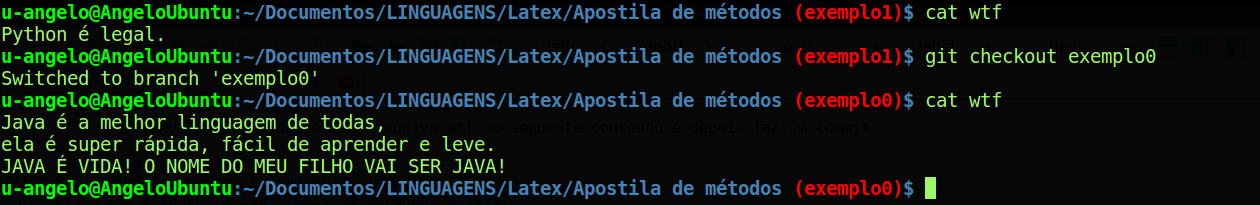
\includegraphics[width=1\linewidth]{conflito1}
	\end{center}
	\legend{Fonte: (Do autor)}
\end{figure}

O desenvolvedor A resolve fazer um \textit{merge} do \textit{branch} do desenvolvedor B, e acaba se deparando com a seguinte mensagem (ver figura \ref{conflito2}): $$\verb|CONFLITO (adicionar/adicionar): conflito de mesclagem em wtf|$$

\begin{figure}[h]
	\caption{\label{conflito2}Resolvendo conflito - parte 2}
	\begin{center}
		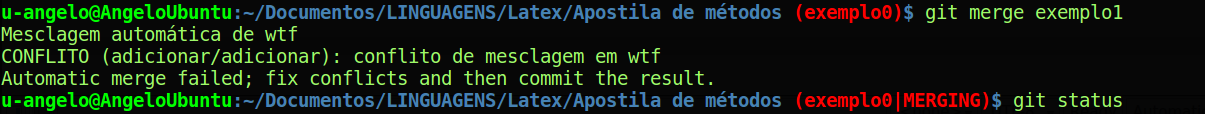
\includegraphics[width=1\linewidth]{conflito2}
	\end{center}
	\legend{Fonte: (Do autor)}
\end{figure}

Se vocês observaram o branch atual após o merge passou a ser \textit{exemplo0|MERGING}. Nessa branch o conteúdo do arquivo wtf (ver figura \ref{conflito3}), é a união dos dois conteúdos, e o desenvolvedor terá que decidir qual código irá permanecer. 

\begin{figure}[h]
	\caption{\label{conflito3}Resolvendo conflito - parte 3}
	\begin{center}
		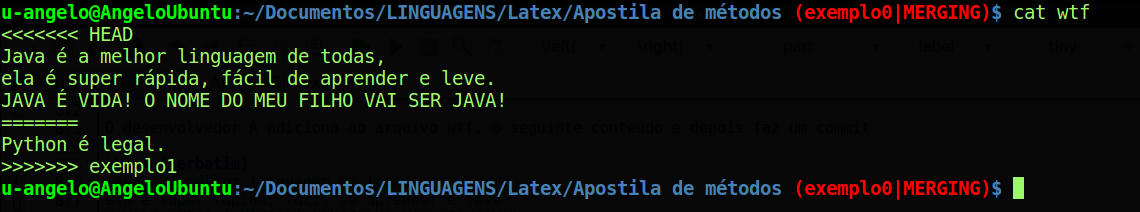
\includegraphics[width=1\linewidth]{conflito3}
	\end{center}
	\legend{Fonte: (Do autor)}
\end{figure}

O desenvolvedor A então edita o arquivo wtf e mantém o conteúdo do desenvolvedor B.  Após alterar o conteúdo ele faz um novo \textit{commit} e, todos os conflito são resolvidos, tanto do código, quanto o ``conflito'' do desenvolvedor A (piada muito boa, eu sei!), ver figura \ref{conflito4}.

\begin{figure}[H]
	\caption{\label{conflito4}Resolvendo conflito - parte 4}
	\begin{center}
		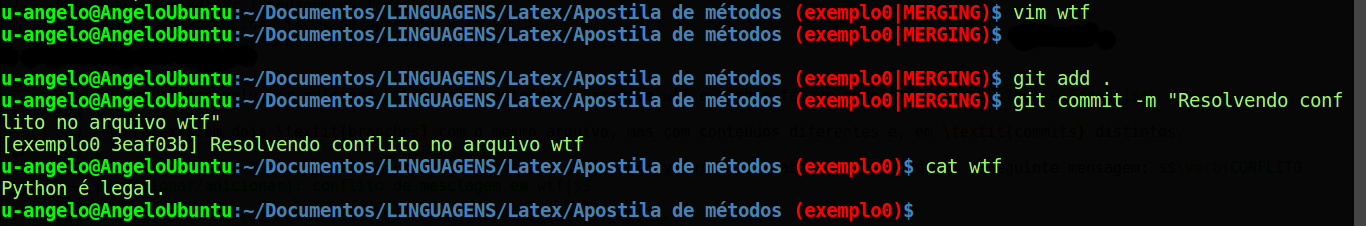
\includegraphics[width=1\linewidth]{conflito4}
	\end{center}
	\legend{Fonte: (Do autor)}
\end{figure}

%%%%%%%%%%%%%%%%%%%%%%%%%%%%%%%%%%%%%%%%%%%%%%%%%%%%%%%%%%%%%%%%

\nocite{book}
\nocite{gitlab}
\nocite{gitflow}
\nocite{semver}
\nocite{gitready}
\nocite{stackoverflow}
\nocite{atlassian}
\nocite{ndpsoftware}
\nocite{rogerdudler}
\nocite{danielkummer}
\nocite{nvie}
\nocite{cgti}
\nocite{moura}
\nocite{wikiversity}
\nocite{stackoverflow2}
\nocite{tribo}
\nocite{devmedia1}
\nocite{devmedia2}
\nocite{marklodato}

%\nocite{eisele}
%\nocite{gille}
%\nocite{carvalho}
%\nocite{cancela}
%\nocite{philippi}
%\nocite{hordonho}
%\nocite{url1}
%\nocite{url2}
%\nocite{born}
%\nocite{costa}
%\nocite{heredia}
%\nocite{christophe}
%\nocite{garcia}
%\nocite{resende}
%\nocite{gois}
%\nocite{rezende}
%\nocite{perovano}
%
\bibliography{biblio}
	 		
\end{document}
